\begin{savequote}[75mm]
Engineering is achieving function while avoiding failure. 
\qauthor{--- Henry Petroski ---}
\end{savequote}

\chapter{Applications of integration}
\label{chap_int_app}
\graphicspath{{figures/Int_App/}}


This chapter employs the following technique to a variety of applications. Suppose the value $Q$ of a quantity is to be calculated. We first approximate the value of $Q$ using a Riemann sum, then find the exact value via a definite integral. This goes as follows.


\begin{enumerate}
\item		Divide the quantity into $n$ smaller subquantities of value $Q_i$.
\item		Identify a variable $x$ and function $f(x)$ such that each subquantity can be approximated with the product $f(c_i)\dx$, where $\dx$ represents a small change in $x$. Thus $Q_i \approx f(c_i)\dx$. A sample approximation $f(c_i)\dx$ of $Q_i$ is called a \textbf{differential element}.
\item		Recognize that $$\ds Q= \sum_{i=1}^n Q_i \approx \sum_{i=1}^n f(c_i)\dx,$$ which is a Riemann Sum.
\item		Taking the appropriate limit gives $Q = \int_a^b f(x)\ dx.$
\end{enumerate}

\section{Area between curves}\label{sec:ABC}
\subsection{Rectangular coordinates}
Let $Q$ be the area of a region bounded by continuous functions $f$ and $g$. If we break the region into many subregions, we have an obvious equation:

\hfill Total area = sum of the areas of the subregions. \hfill \null

The issue to address next is how to systematically break a region into subregions. Consider Figure \ref{fig_int_app_1a}  where a region between two curves is shaded. While there are many ways to break this into subregions, one particularly efficient way is to slice it vertically, as shown in Figure \ref{fig_int_app_1b}, into $n$ equally spaced slices. 

\begin{figure}[H]
\centering
%\raisebox{0.5cm}{
\subfigure[\label{fig_int_app_1a}]{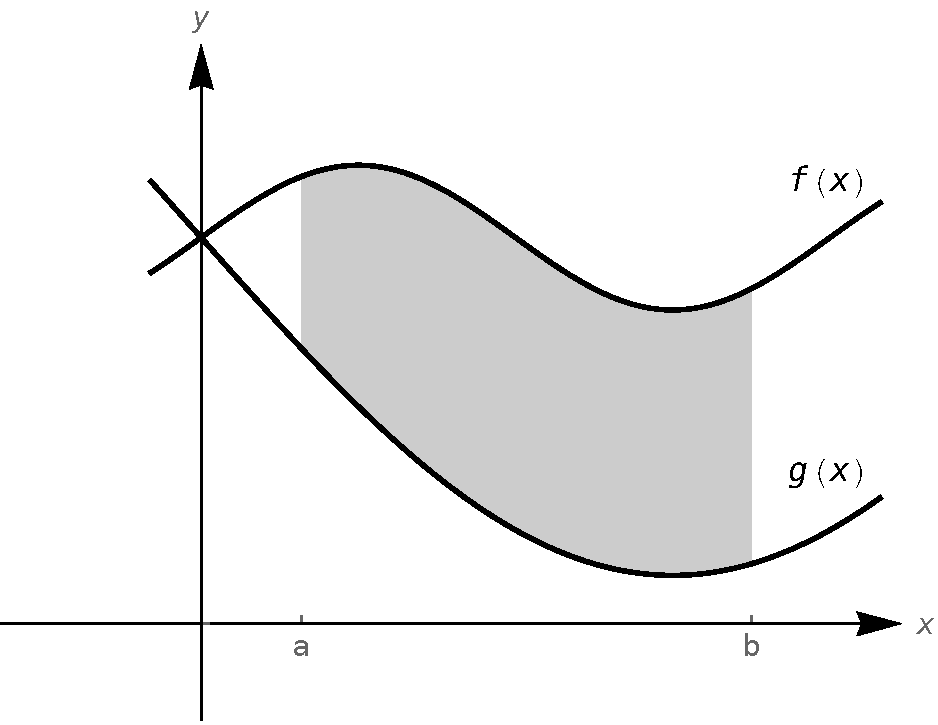
\includegraphics[width=0.4\textwidth]{fig_int_app_1a}}
\qquad
\subfigure[\label{fig_int_app_1b}]{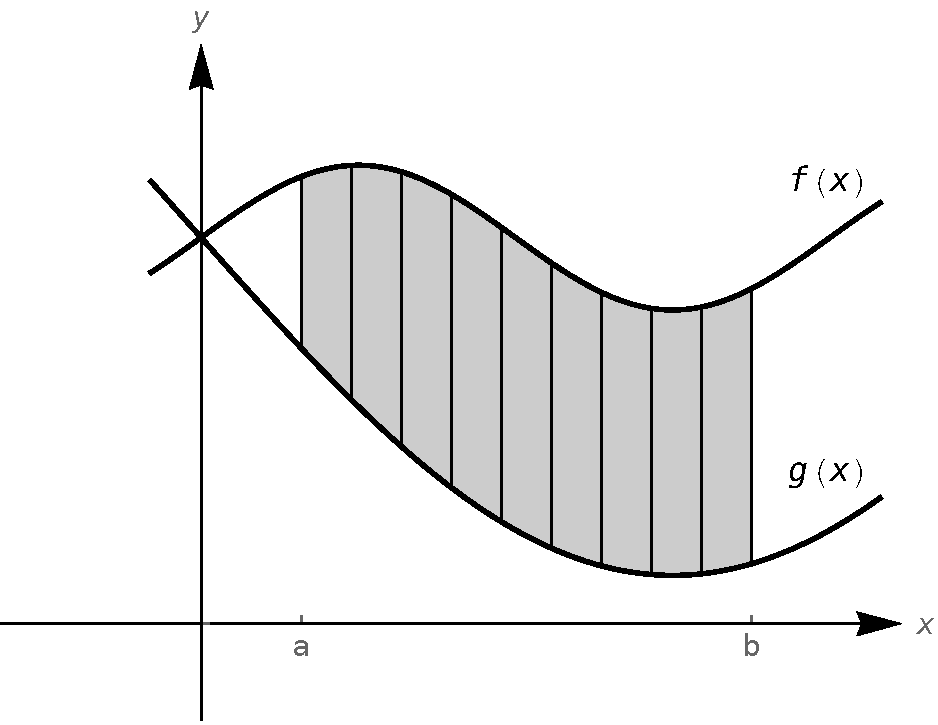
\includegraphics[width=0.4\textwidth]{fig_int_app_1b} }
\qquad
\subfigure[\label{fig_int_app_1c}]{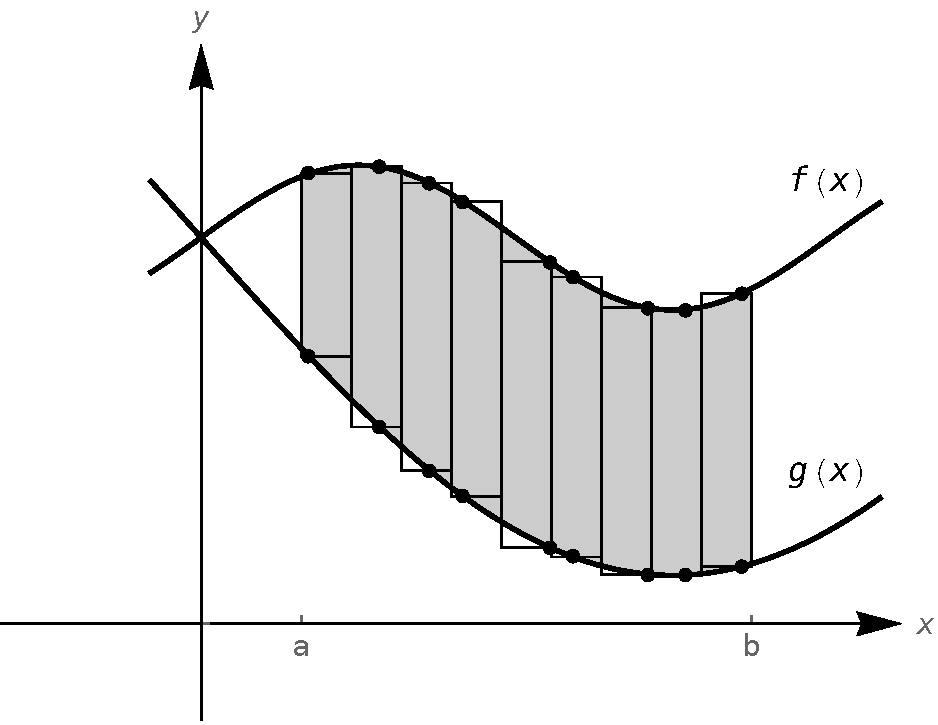
\includegraphics[width=0.4\textwidth]{fig_int_app_1c} }
\caption{Subdividing a region into vertical slices and approximating the areas with rectangles.}
\end{figure}


We now approximate the area of a slice. Again, we have many options, but using a rectangle seems simplest. Picking any $x$-value $c_i$ in the $i^\text{ th}$ slice, we set the height of the rectangle to be $f(c_i)-g(c_i)$, the difference of the corresponding $y$-values. The width of the rectangle is a small difference in $x$-values, which we represent with $\dx$. Figure \ref{fig_int_app_1c}  shows sample points $c_i$ chosen in each subinterval and appropriate rectangles drawn. Each of these rectangles represents a differential element. Each slice has an area approximately equal to $\big(f(c_i)-g(c_i)\big)\dx$; hence, the total area is approximately the Riemann sum
$$Q = \sum_{i=1}^n \big(f(c_i)-g(c_i)\big)\dx.$$
Taking the limit as $n\to +\infty$ gives the exact area $A$ as 
\begin{equation}
\ds\int\limits_a^b \big(f(x)-g(x)\big)\ dx.
\label{eq_area}
\end{equation}

\begin{example}\label{ex_abc2}
Find the total area of the region enclosed by the functions $f(x) = -2x+5$ and \\ $g(x) = x^3-7x^2+12x-3$ as shown in Figure \ref{fig_int_app_2}.


\begin{figure}[H]
	\begin{center}
			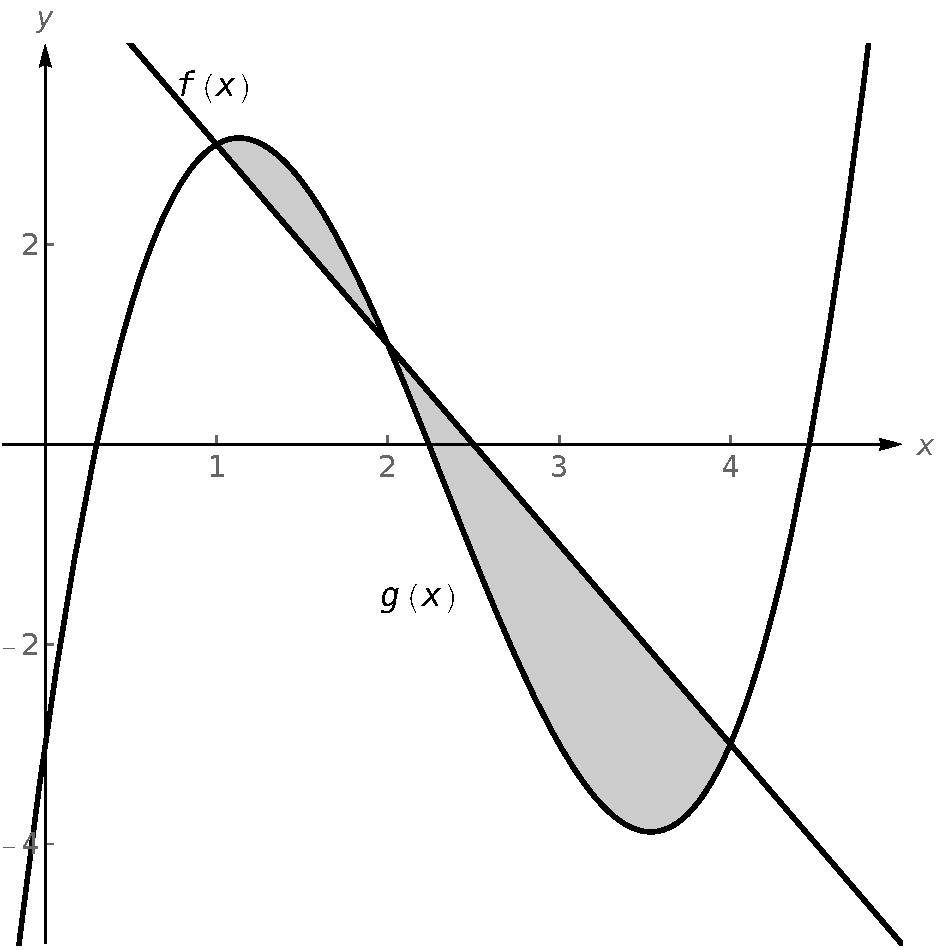
\includegraphics[width=0.4\textwidth]{fig_int_app_2}
	\caption{Graphing a region enclosed by two functions in Example \ref{ex_abc2}.}
	\label{fig_int_app_2}
	\end{center}
\end{figure}

\xhrulefill{gray}{2.5pt}Solution \xhrulefill{gray}{2.5pt}

A quick calculation shows that $f=g$ at $x=1, 2$ and 4. One can proceed thoughtlessly by computing $ \int_1^4\big(f(x)-g(x)\big)\ dx$, but this ignores the fact that on $[1,2]$, $g(x)>f(x)$.  Thus we compute the total area by breaking the interval $[1,4]$ into two subintervals, $[1,2]$ and $[2,4]$ and using the proper integrand in each.
\begin{align*}
\text{Total Area} &= \ds\int\limits_1^2 \big(g(x)-f(x)\big)\ dx + \ds\int\limits_2^4\big(f(x)-g(x)\big)\ dx\\[0.2cm]
			&= \ds\int\limits_1^2 \big(x^3-7x^2+14x-8\big) \ dx + \ds\int\limits_2^4\big(-x^3+7x^2-14x+8\big)\ dx\\[0.2cm]
			&= \dfrac{5}{12} + \dfrac{8}{3} \\
			&= \dfrac{37}{12} = 3.083\ \text{units}^2.
\end{align*}		
\end{example}

The previous example makes note that we are expecting area to be positive. When first learning about the definite integral, we interpreted it as signed area under the curve, allowing for negative area. That does not apply here; area is to be positive.

The previous example also demonstrates that we often have to break a given region into subregions. The following example shows another situation where this is applicable.

\begin{example}\label{ex_abc3}
Find the area of the region enclosed by the functions $y=\sqrt{x}+2$, $y=-(x-1)^2+3$ and $y=2$, as shown in Figure \ref{fig_int_app_3a}.


\pagebreak

\xhrulefill{gray}{2.5pt}Solution \xhrulefill{gray}{2.5pt}

We give two approaches to this problem. In the first approach, we notice that the region's top is defined by two different curves. On $[0,1]$, the top function is $y=\sqrt{x}+2$; on $[1,2]$, the top function is $y=-(x-1)^2+3$. 

Thus we compute the area as the sum of two integrals:
\begin{align*}
\text{A} &= \ds\int\limits_0^1 \Big(\big(\sqrt{x}+2\big)-2\Big)\ dx + \ds\int\limits_1^2 \Big(\big(-(x-1)^2+3\big)-2\Big)\ dx \\
									&= \dfrac{2}{3}+\dfrac{2}{3}\\
									&=\dfrac{4}{3}.
\end{align*}


\begin{figure}[H]
\centering
%\raisebox{0.5cm}{
\subfigure[\label{fig_int_app_3a}]{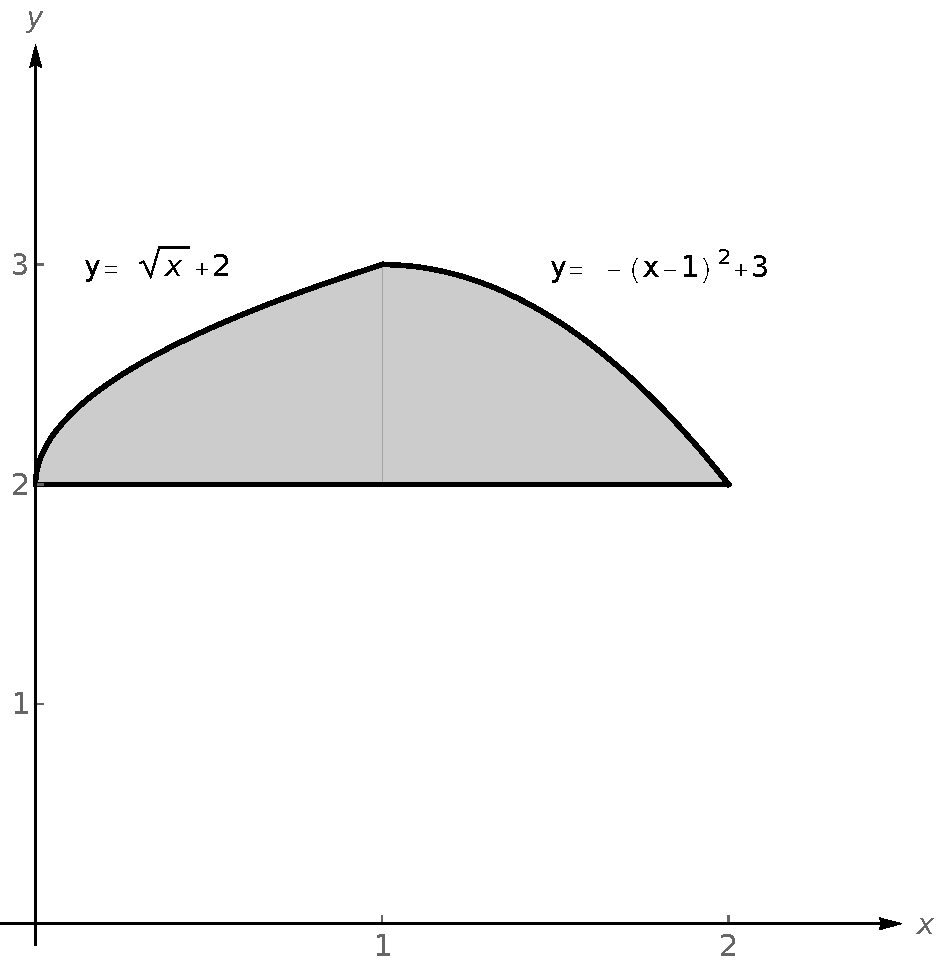
\includegraphics[width=0.45\textwidth]{fig_int_app_3a}}
\qquad
\subfigure[\label{fig_int_app_3b}]{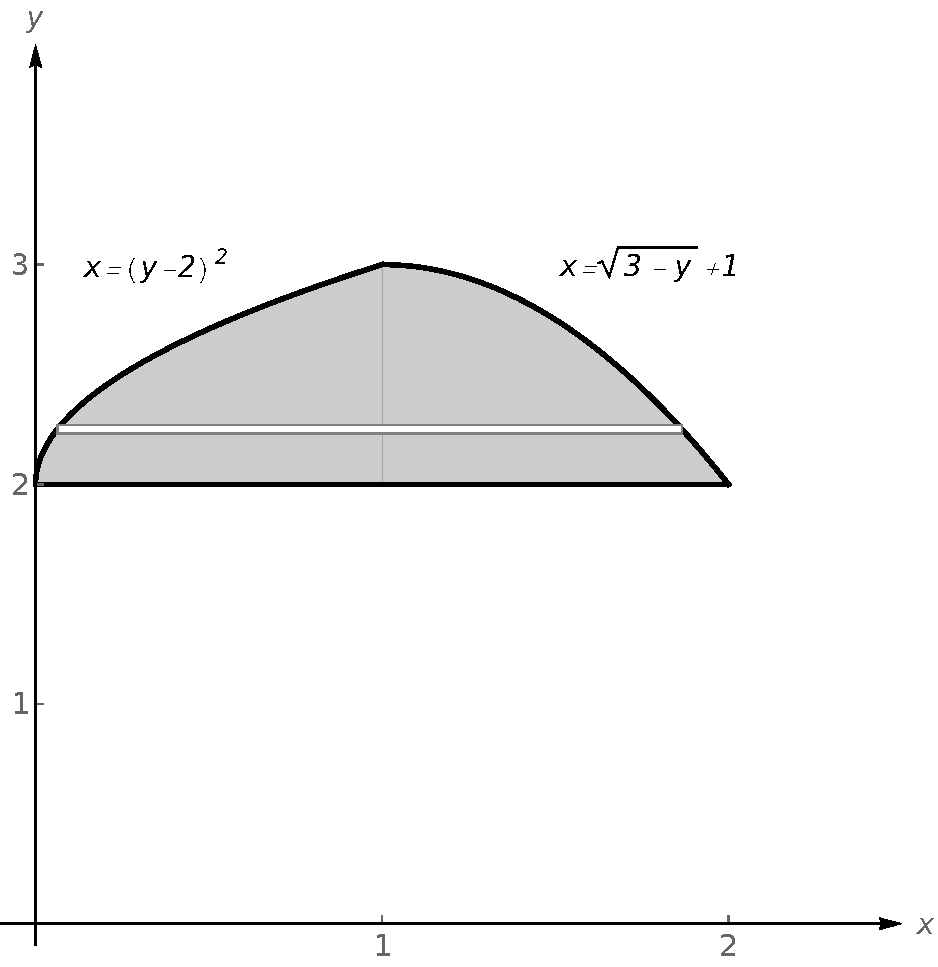
\includegraphics[width=0.45\textwidth]{fig_int_app_3b} }
\caption{Graphing a region for Example \ref{ex_abc3} (a) and the region with boundaries relabelled as functions of $y$ (b).}
\end{figure}


The second approach is clever and very useful in certain situations. We are used to viewing curves as functions of $x$; we input an $x$-value and a $y$-value is returned. Some curves can also be described as functions of $y$: input a $y$-value and an $x$-value is returned. We can rewrite the equations describing the boundary by solving for $x$:
	$$y=\sqrt{x}+2 \quad \Rightarrow\quad x=(y-2)^2$$
	$$y=-(x-1)^2+3 \quad \Rightarrow \quad x=\sqrt{3-y}+1.$$


Figure \ref{fig_int_app_3b} shows the region with the boundaries relabelled. A differential element, a horizontal rectangle, is also pictured.	The width of the rectangle is a small change in $y$: $\Delta y$. The height of the rectangle is a difference in $x$-values. The top $x$-value is the largest value, i.e., the rightmost. The bottom $x$-value is the smaller, i.e., the leftmost. Therefore the height of the rectangle is $$\big(\sqrt{3-y}+1\big) - (y-2)^2.$$

The area is found by integrating the above function with respect to $y$ with the appropriate bounds. We determine these by considering the $y$-values the region occupies. It is bounded below by $y=2$, and bounded above by $y=3$. That is, both the top and bottom functions exist on the $y$ interval $[2,3]$. Thus
\begin{align*}
\text{A} &= \ds\int\limits_2^3 \Big(\sqrt{3-y}+1 - (y-2)^2\Big)\ dy \\[0.2cm]
			&= \Big(-\frac23(3-y)^{3/2}+y-\frac13(y-2)^3\Big)\Big|_2^3 \\[0.2cm]
			&= \dfrac{4}{3}.
\end{align*}



\end{example}

While we have focused on producing exact answers, we are also able to make approximations. The integrand in Equation~\eqref{eq_area} is a distance (top minus bottom); integrating this distance function gives an area. By taking discrete measurements of distance, we can approximate an area using numerical integration techniques developed in Chapter~\ref{chap_int}.


% The following example demonstrates this.
%
%\begin{example}\label{ex_abc5}
%To approximate the area of a lake, shown in Figure \ref{fig_int_app_4a},  the length of the lake is measured at 200-meters increments as shown in Figure \ref{fig_int_app_4b}, where the lengths are given in hundreds of metres. Approximate the area of the lake.
%
%\xhrulefill{gray}{2.5pt}Solution \xhrulefill{gray}{2.5pt}
%
%The measurements of length can be viewed as measuring top minus bottom of two functions. The exact answer is found by integrating $ \int_0^{12} \big(f(x)-g(x)\big)\ dx$, but of course we do not know the functions $f$ and $g$. Our discrete measurements instead allow us to approximate.
%
%We have the following data points:
%$$(0,0),\ (2,2.25),\ (4,5.08),\ (6,6.35),\ (8,5.21),\ (10,2.76),\ (12,0).$$
%We also have that $\dx=\frac{b-a}{n} = 2$, so Simpson's rule gives
%\begin{align*}
%\text{Area}&\approx \frac{2}{3}\Big(1\cdot0+4\cdot2.25+2\cdot5.08+4\cdot6.35+2\cdot5.21+4\cdot2.76+1\cdot0\Big)\\
%			&= 44.01\overline{3} \ \text{units}^2.
%\end{align*}
%
%Since the measurements are in hundreds of metres, units$^2 = (100\ \text{m})^2 = 10,000\ \text{m}^2$, giving a total area of $440,133\ \text{m}^2$. 
%
%\begin{figure}[H]
%\centering
%%\raisebox{0.5cm}{
%\subfigure[\label{fig_int_app_4a}]{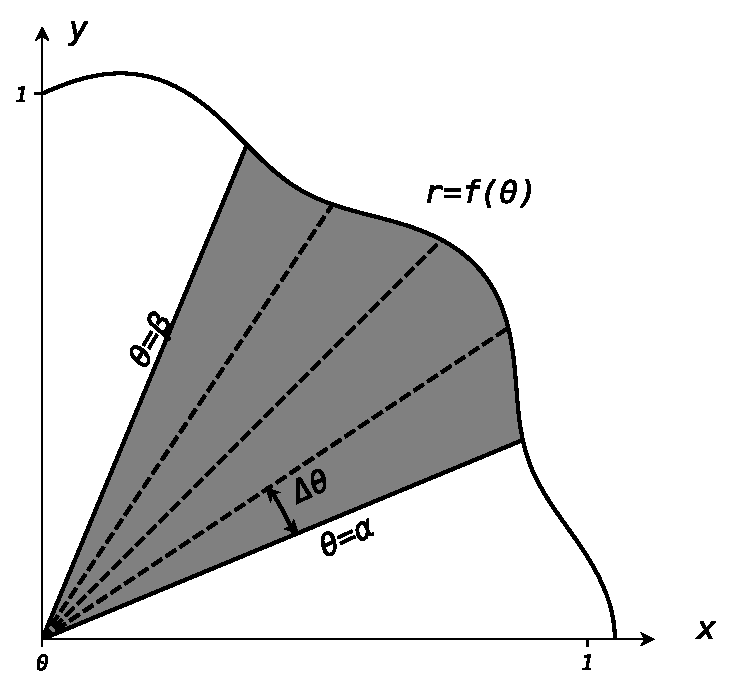
\includegraphics[width=0.45\textwidth]{fig_int_app_4a}}
%\qquad
%\subfigure[\label{fig_int_app_4b}]{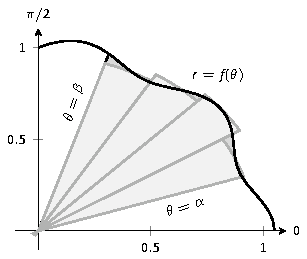
\includegraphics[width=0.45\textwidth]{fig_int_app_4b} }
%\caption{A sketch of a lake (a) , and  the lake with length measurements (b).}
%\end{figure}
%
%\end{example}

In the next section we apply our applications--of--integration techniques to finding the volumes of certain solids.

\subsection{Polar coordinates}
\checkoddpage
\marginpar{\ifoddpage\hspace*{-1.5cm}\else\hspace*{0.25cm}\fi
\includegraphics[width=0.075\textwidth]{youtube}\\
\ifoddpage\hspace*{-1.75cm}\else\hspace*{0.1cm}\fi
\qrcode[height=1.75cm]{https://youtu.be/qVn_Lfec-Ac}
%\includegraphics[width=0.1\textwidth]{polar_cor_int}
}
When using polar coordinates, the equations $\theta=\alpha$ form lines through the origin and $r=c$ form circles centred at the origin, respectively, and combinations of these curves form sectors of circles. It is then somewhat natural to calculate the area of regions defined by polar functions by first approximating with sectors of circles. 

Consider Figure \ref{fig_int_app_4a}  where a region defined by $r=f(\theta)$ on $[\alpha,\beta]$ is given. Note how the sides of the region are the lines $\theta=\alpha$ and $\theta=\beta$, whereas in rectangular coordinates the sides of regions were often the vertical lines $x=a$ and $x=b$. 

Partition the interval $[\alpha,\beta]$ into $n$ equally spaced subintervals as $\alpha = \theta_1 < \theta_2 <\cdots <\theta_{n+1}=\beta$. The length of each subinterval is $\Delta\theta = (\beta-\alpha)/n$, representing a small change in angle. The area of the region defined by the $i\,^\text{th}$ subinterval $[\theta_i,\theta_{i+1}]$ can be approximated with a sector of a circle with radius $f(c_i)$, for some $c_i$ in $[\theta_i,\theta_{i+1}]$. The area of this sector is $\frac12f(c_i)^2\Delta\theta$. This is shown in Figure~\ref{fig_int_app_4b}, where $[\alpha,\beta]$ has been divided into 4 subintervals. We approximate the area of the whole region by summing the areas of all sectors:
$$\text{Area} \approx \sum_{i=1}^n \frac12f(c_i)^2\Delta\theta.$$
This is a Riemann sum. By taking the limit of the sum as $n\to +\infty$, we find the exact area of the region in the form of a definite integral:
\begin{equation}
A \ =\  \frac12\int\limits_\alpha^\beta f(\theta)^2 \ d\theta\  =\  \frac12\int\limits_\alpha^\beta r^{\,2} \ d\theta.
\label{thm:polar_area}
\end{equation}

By having $0\leq \beta-\alpha\leq 2\pi$, we ensure that the region does not overlap itself, which would give a result that does not correspond directly to the area.

\begin{figure}[h]
\centering
%\raisebox{0.5cm}{
\subfigure[\label{fig_int_app_4a}]{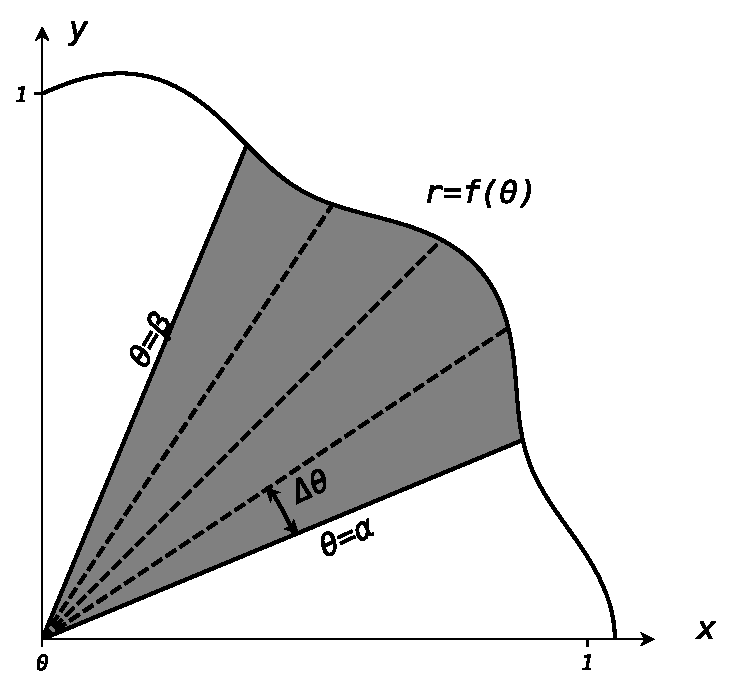
\includegraphics[width=0.45\textwidth]{fig_int_app_4a}}
\qquad
\subfigure[\label{fig_int_app_4b}]{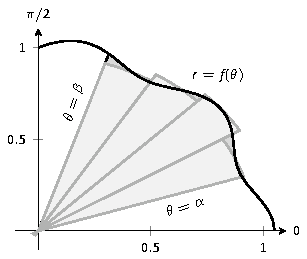
\includegraphics[width=0.45\textwidth]{fig_int_app_4b} }
\caption{Computing the area of a polar region.}
\end{figure}

\begin{example}\label{ex_polcalc4}
Find the area of the cardioid $r=1+\cos(\theta)$ bound between $\theta=\pi/6$ and $\theta=\pi/3$, as shown in Figure \ref{fig_int_app_5}.

\begin{figure}[H]
	\begin{center}
			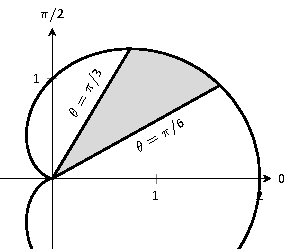
\includegraphics[width=0.4\textwidth]{fig_int_app_5}
	\caption{Finding the area of the shaded region of a cardioid in Example \ref{ex_polcalc4}.}
	\label{fig_int_app_5}
	\end{center}
\end{figure}

\xhrulefill{gray}{2.5pt}Solution \xhrulefill{gray}{2.5pt}

This is a direct application of Equation~\eqref{thm:polar_area}. 
\allowdisplaybreaks
\begin{align*}
\text{Area} &= \frac12\int\limits_{\pi/6}^{\pi/3} (1+\cos(\theta))^2\ d\theta\\[0.2cm]
				&= \frac12\int\limits_{\pi/6}^{\pi/3} (1+2\cos(\theta)+\cos^2(\theta))\ d\theta\\[0.2cm]
				&= \frac12\left(\theta+2\sin(\theta)+\frac12\theta+\frac14\sin(2\theta)\right)\Bigg|_{\pi/6}^{\pi/3} \\[0.2cm]
				&= \frac18\big(\pi+4\sqrt{3}-4\big) \approx 0.7587
				\end{align*}
				



\end{example}


We may of course also determine the region enclosed between two polar curves. Consider for that purpose the shaded region shown in Figure \ref{fig_int_app_6}. We can find the area of this region by computing the area bounded by $r_2=f_2(\theta)$ and subtracting the area bounded by $r_1=f_1(\theta)$ on $[\alpha,\beta]$. Thus
\begin{equation}
\text{Area}\ = \ \frac12\int\limits_\alpha^\beta r_2^{\,2}\ d\theta - \frac12\int\limits_\alpha^\beta r_1^{\,2}\ d\theta = \frac12\int\limits_\alpha^\beta \big(r_2^{\,2}-r_1^{\,2}\big)\ d\theta.
\label{idea:area_between_polar}
\end{equation}

\begin{figure}[H]
	\begin{center}
			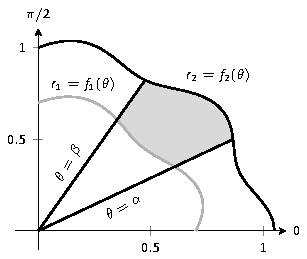
\includegraphics[width=0.5\textwidth]{fig_int_app_6}
	\caption{Illustrating area bound between two polar curves.}
	\label{fig_int_app_6}
	\end{center}
\end{figure}

\begin{example}\label{ex_polcalc6}
Find the area bounded between the polar curves $r=1$ and $r=2\cos(2\theta)$, as shown in Figure \ref{fig_int_app_7a}.



\xhrulefill{gray}{2.5pt}Solution \xhrulefill{gray}{2.5pt}

We need to find the point of intersection between the two curves. Setting the two functions equal to each other, we have
$$2\cos(2\theta) = 1 \quad \Leftrightarrow \quad \cos(2\theta) = \frac12 \quad \Rightarrow \quad 2\theta = \dfrac{\pi}{3}\quad \Rightarrow \quad \theta=\dfrac{\pi}{6}.$$

In Figure~\ref{fig_int_app_7b}, we zoom in on the region and note that it is not really bounded between two polar curves, but rather by two polar curves, along with $\theta=0$. The dashed line breaks the region into its component parts. Below the dashed line, the region is defined by $r=1$, $\theta=0$ and $\theta = \pi/6$. Above the dashed line the region is bounded by $r=2\cos(2\theta)$ and $\theta =\pi/6$. Since we have two separate regions, we find the area using two separate integrals.

Call the area below the dashed line $A_1$ and the area above the dashed line $A_2$. They are determined by the following integrals:
$$A_1 = \frac12\int\limits_0^{\pi/6} (1)^2\ d\theta \qquad \text{and} \qquad A_2 = \frac12\int\limits_{\pi/6}^{\pi/4} \big(2\cos(2\theta)\big)^2\ d\theta.$$
The upper bound of the integral for $A_2$ is $\pi/4$ as $r=2\cos(2\theta)$ is at the pole when $\theta=\pi/4$.
We omit the integration details and let the reader verify that $A_1 = \pi/12$ and $A_2 = \pi/12-\sqrt{3}/8$; the total area is $A = \pi/6-\sqrt{3}/8$.

\begin{figure}[H]
\centering
%\raisebox{0.5cm}{
\subfigure[\label{fig_int_app_7a}]{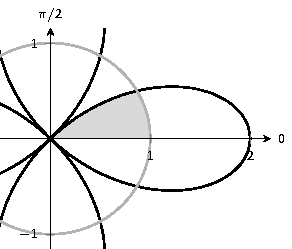
\includegraphics[width=0.45\textwidth]{fig_int_app_7a}}
\qquad
\subfigure[\label{fig_int_app_7b}]{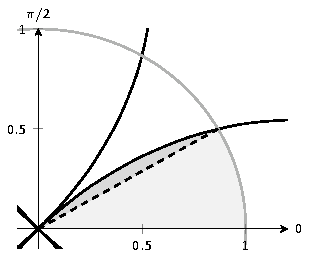
\includegraphics[width=0.45\textwidth]{fig_int_app_7b} }
\caption{Graphing the region bounded by the functions in Example \ref{ex_polcalc6}.}
\end{figure}


\end{example}

\begin{remark}[The error function]
The error function is an example of a non-elementary function that contains an integral in its definition.  More precisely,  it is defined as:
$$
\displaystyle {\begin{aligned}\operatorname {erf} (x)&={\frac {1}{\sqrt {\pi }}}\int\limits _{-x}^{x}e^{-t^{2}}\,dt={\frac {2}{\sqrt {\pi }}}\int\limits _{0}^{x}e^{-t^{2}}\,dt.\end{aligned}}
$$
It is of sigmoid shape and  occurs in probability and statistic (Figure~\ref{fig_int_app_8}). There, for nonnegative values of $x$, it has the following interpretation: for a random variable Y that is normally distributed with mean 0 and variance 1/2, $\text{erf}(x)$ describes the probability of $Y$ falling in the range $[-x, x]$. 

\begin{figure}[H]
	\begin{center}
			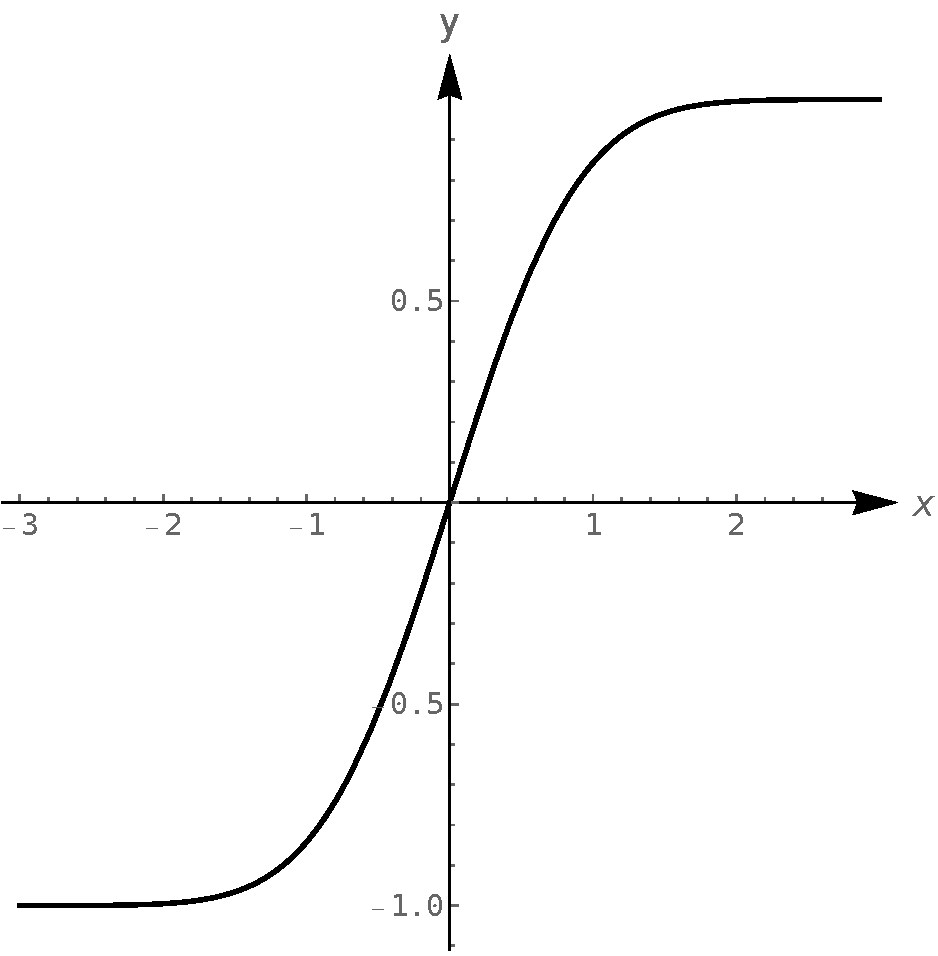
\includegraphics[width=0.25\textwidth]{fig_int_app_8}
	\caption{A graph of the error function.}
	\label{fig_int_app_8}
	\end{center}
\end{figure}


\end{remark}

\section{Volume by cross-sectional area}\label{sec:disk}

\subsection{Volumes by slicing}
The volume of a general right cylinder, as shown in Figure \ref{fig_int_app_9}, is 

\hfill Area of the base $\times$ height. \hfill\null

We can use this fact as the building block in finding volumes of a variety of shapes.


\begin{figure}[h]
	\begin{center}
			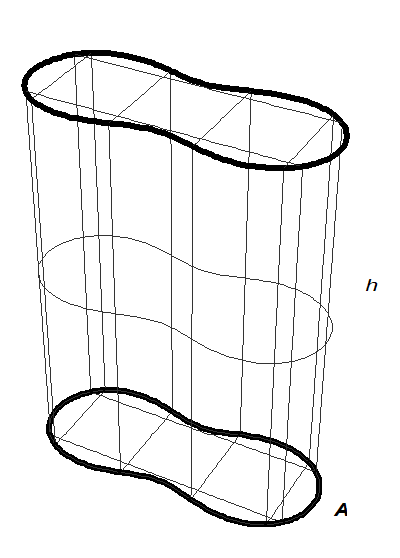
\includegraphics[width=0.4\textwidth]{fig_int_app_9.png}
	\caption{The volume of a general right cylinder.}
	\label{fig_int_app_9}
	\end{center}
\end{figure}

Given an arbitrary solid, we can approximate its volume by cutting it into $n$  thin slices. When the slices are thin, each slice can be approximated well by a general right cylinder. Thus the volume of each slice is approximately its cross-sectional area $\times$ thickness. These slices are the differential elements.

By orienting a solid along the $x$-axis, we can let $A(x_i)$ represent the cross-sectional area
of the $i\,^\text{th}$ slice, and let $\dx_i$ represent the thickness of this slice. The total volume of the solid is approximately:
	\begin{align*} \text{Volume} &\approx \sum_{i=1}^n \Big[\text{Area}\ \times\ \text{thickness}\Big] \\
			&= \sum_{i=1}^n A(x_i)\dx_i.
	\end{align*}
	
Recognize that this is a Riemann sum. By taking a limit as the thickness of the slices goes to 0 we can find the volume exactly. 

\pagebreak
\begin{theorem}[Volume by cross-sectional area]\label{thm:volume_by_cross_section}
The volume $V$ of a solid, oriented along the $x$-axis with cross-sectional area $A(x)$ from $x=a$ to $x=b$, is 
$$V = \int\limits_a^b A(x)\ dx.$$
\end{theorem}




\begin{example}\label{ex_disk0}
Find the volume of a pyramid with a square base of side length 10 cm and a height of 5 cm.

\xhrulefill{gray}{2.5pt}Solution \xhrulefill{gray}{2.5pt}

There are many ways to orient the pyramid along the $x$-axis; Figure \ref{fig_int_app_10a} gives one such way, with the pointed top of the pyramid at the origin and the $x$-axis going through the centre of the base.


Each cross section of the pyramid is a square; this is a sample differential element. To determine its area $A(x)$, we need to determine the side lengths of the square.
When $x=5$, the square has side length 10; when $x=0$, the square has side length 0. Since the edges of the pyramid are lines, it is easy to figure that each cross-sectional square has side length $2x$, giving $A(x) = (2x)^2=4x^2$. % 

If one were to cut a slice out of the pyramid at $x=3$, as shown in Figure \ref{fig_int_app_10b}, one would have a shape with square bottom and top with sloped sides. If the slice were thin, both the bottom and top squares would have sides lengths of about 6, and thus the cross--sectional area of the bottom and top would be about 36cm$^2$. Letting $\Delta x_i$ represent the thickness of the slice, the volume of this slice would then be about $36\Delta x_i$ cm$^3$. 

Cutting the pyramid into $n$ slices divides the total volume into $n$ equally--spaced smaller pieces, each with volume $(2x_i)^2\Delta x$, where $x_i$ is the approximate location of the slice along the $x$-axis and $\Delta x$ represents the thickness of each slice. One can approximate the total volume of the pyramid by summing up the volumes of these slices:
$$\text{Approximate volume } = \sum_{i=1}^n (2x_i)^2\Delta x.$$
Taking the limit as $n\to+\infty$ gives the actual volume of the pyramid; recognizing this sum as a Riemann sum allows us to find the exact answer using a definite integral, matching the definite integral given by Theorem \ref{thm:volume_by_cross_section}.

We have 
\allowdisplaybreaks
\begin{align*} V &= \lim_{n\to+\infty} \sum_{i=1}^n (2x_i)^2\Delta x\\[0.2cm]
							&= \int\limits_0^5 4x^2\ dx\\[0.2cm]
				&= \frac43x^3\Big|_0^5 \\[0.2cm]
				&=\frac{500}{3}\ \text{in}^3 \approx 166.67\ \text{cm}^3.
\end{align*}
\begin{figure}[H]
\centering
%\raisebox{0.5cm}{
\subfigure[\label{fig_int_app_10a}]{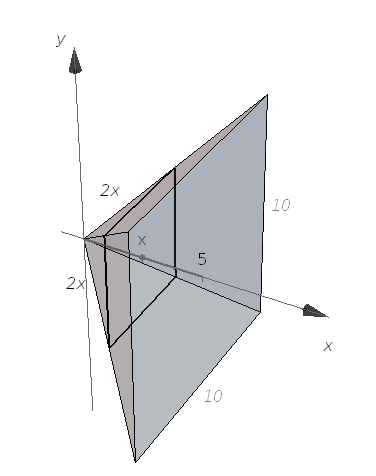
\includegraphics[width=0.45\textwidth]{fig_int_app_10a}}
\qquad
\subfigure[\label{fig_int_app_10b}]{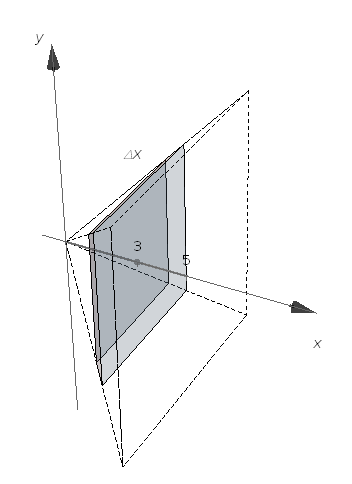
\includegraphics[width=0.45\textwidth]{fig_int_app_10b} }
\caption{Orienting a pyramid along the $x$-axis (a) and cutting a slice in it at $x=3$ (b) in Example \ref{ex_disk0}.}
\end{figure}

\end{example}

\subsection{Solids of revolution}
\ifcalculus
\checkoddpage
\marginpar{\ifoddpage\hspace*{-1.5cm}\else\hspace*{0.25cm}\fi
\includegraphics[width=0.075\textwidth]{youtube}\\
\ifoddpage\hspace*{-1.75cm}\else\hspace*{0.1cm}\fi
\qrcode[height=1.75cm]{https://youtu.be/Thvc2s9aUP4}
%\includegraphics[width=0.1\textwidth]{snede_ing}
}
\fi
\ifanalysis
\checkoddpage
\marginpar{\ifoddpage\hspace*{-1.5cm}\else\hspace*{0.25cm}\fi
\includegraphics[width=0.075\textwidth]{youtube}\\
\ifoddpage\hspace*{-1.75cm}\else\hspace*{0.1cm}\fi
\qrcode[height=1.75cm]{https://youtu.be/OFNGpKGg9IQ}
%\includegraphics[width=0.1\textwidth]{snede_ir}
}
\fi
An important special case of Theorem \ref{thm:volume_by_cross_section} is when the solid is a \textbf{solid of revolution} (\textit{omwente\-lingslichaam}), that is, when the solid is formed by rotating a shape about an axis. \index{solid of revolution}\index[aut]{omwentelingslichaam}

Start with a function $y=f(x)$ from $x=a$ to $x=b$. Revolving this curve about a horizontal axis creates a three-dimensional solid whose cross sections are disks (thin circles). Let $R(x)$ represent the radius of the cross-sectional disk at $x$; the area of this disk is $\pi R(x)^2$. Applying Theorem \ref{thm:volume_by_cross_section} gives the disk method.



More precisely, let a solid be formed by revolving the curve $y=f(x)$ from $x=a$ to $x=b$ about a horizontal axis, and let $R(x)$ be the radius of the cross-sectional disk at $x$. The volume of the resulting solid is
\index{integration!disk method}\index{disk method}
\begin{equation}
V = \pi \int\limits_a^b R(x)^2\ dx.
\label{idea:disk_method}
\end{equation}

\begin{example}\label{ex_disk1}
Find the volume of the solid formed by revolving the curve $y=1/x$, from $x=1$ to $x=2$, about the $x$-axis.

\xhrulefill{gray}{2.5pt}Solution \xhrulefill{gray}{2.5pt}

A sketch can help us understand this problem. In Figure \ref{fig_int_app_11a} the curve $y=1/x$ is sketched along with the differential element -- a disk -- at $x$ with radius $R(x)=1/x$. In Figure \ref{fig_int_app_11b} the whole solid is pictured, along with the differential element. 

\begin{figure}[H]
\centering
%\raisebox{0.5cm}{
\subfigure[\label{fig_int_app_11a}]{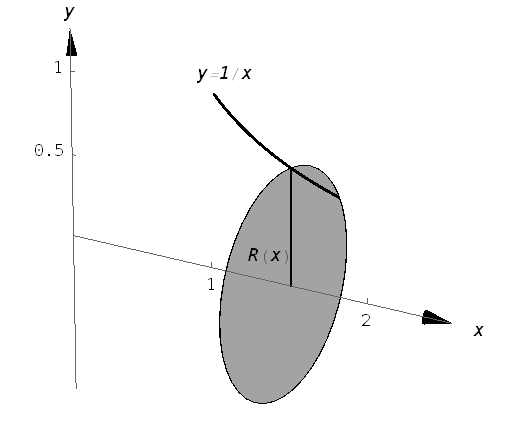
\includegraphics[width=0.45\textwidth]{fig_int_app_11a}}
\qquad
\subfigure[\label{fig_int_app_11b}]{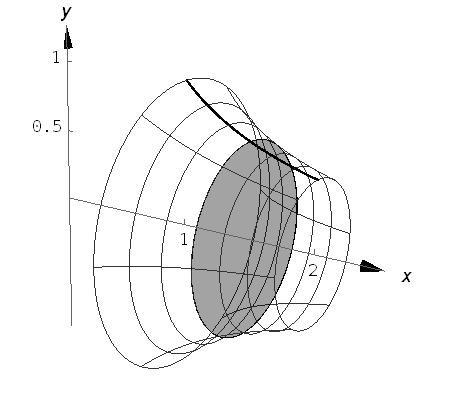
\includegraphics[width=0.45\textwidth]{fig_int_app_11b} }
\caption{Sketching a solid in Example \ref{ex_disk1}.}
\end{figure}

The volume of the differential element shown in part (a) of the figure is approximately $\pi R(x_i)^2\Delta x$, where $R(x_i)$ is the radius of the disk shown and $\Delta x$ is the thickness of that slice. The radius $R(x_i)$ is the distance from the $x$-axis to the curve, hence $R(x_i) = 1/x_i$.



Slicing the solid into $n$ equally--spaced slices, we can approximate the total volume by adding up the approximate volume of each slice:
$$\text{Approximate volume } = \sum_{i=1}^n \pi \left(\frac1{x_i}\right)^2\Delta x.$$

Taking the limit of the above sum as $n\to+\infty$ gives the actual volume; recognizing this sum as a Riemann sum allows us to evaluate the limit with a definite integral, which matches Equation~\eqref{idea:disk_method}:

%Using Key Idea \ref{idea:disk_method}, we have 
\allowdisplaybreaks
\begin{align*}
	V &= \lim_{n\to+\infty}\sum_{i=1}^n \pi \left(\frac1{x_i}\right)^2\Delta x\\[0.2cm]
		&= \pi\int\limits_1^2 \left(\frac1x\right)^2\ dx \\[0.2cm]
		&= \pi\int\limits_1^2 \frac1{x^2}\ dx\\[0.2cm]
		&= \pi\left[-\frac1x\right]\Bigg|_1^2 \\
		&= \pi \left[-\frac12 - \left(-1\right)\right] \\
		&= \frac{\pi}{2}\ \text{units}^3.
\end{align*}





\end{example}


While Equation~\eqref{idea:disk_method} is given in terms of functions of $x$, the principle involved can be as well applied to functions of $y$ when the axis of rotation is vertical, not horizontal. We demonstrate this in the next example.

\begin{example}\label{ex_disk2}
Find the volume of the solid formed by revolving the curve $y=1/x$, from $x=1$ to $x=2$, about the $y$-axis.

\xhrulefill{gray}{2.5pt}Solution \xhrulefill{gray}{2.5pt}

Since the axis of rotation is vertical, we need to convert the function into a function of $y$ and convert the $x$-bounds to $y$-bounds. Since $y=1/x$ defines the curve, we rewrite it as $x=1/y$. The bound $x=1$ corresponds to the $y$-bound $y=1$, and the bound $x=2$ corresponds to the $y$-bound $y=1/2$. 
Thus we are rotating the curve $x=1/y$, from $y=1/2$ to $y=1$ about the $y$-axis to form a solid. The curve and sample differential element are sketched in Figure \ref{fig_int_app_12a}, with a full sketch of the solid in Figure \ref{fig_int_app_12b}.


\begin{figure}[H]
\centering
%\raisebox{0.5cm}{
\subfigure[\label{fig_int_app_12a}]{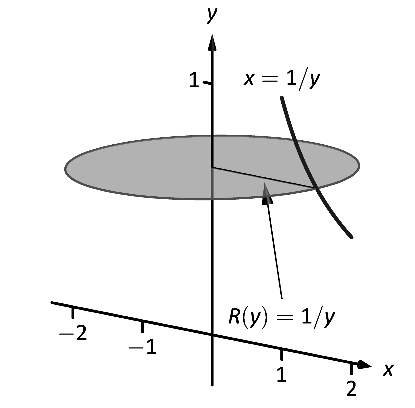
\includegraphics[width=0.45\textwidth]{fig_int_app_12a}}
\qquad
\subfigure[\label{fig_int_app_12b}]{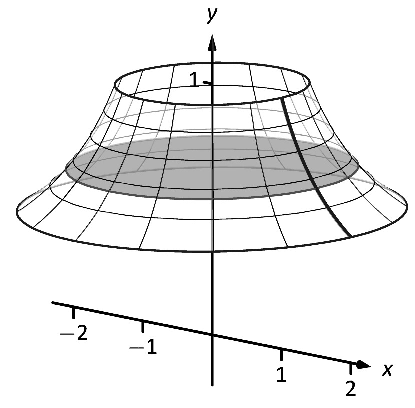
\includegraphics[width=0.45\textwidth]{fig_int_app_12b} }
\caption{Sketching a solid in Example \ref{ex_disk2}.}
\end{figure}



We integrate to find the volume:
\begin{align*}
V &= \pi\int\limits_{1/2}^1 \frac{1}{y^2}\ dy \\[0.2cm]
	&= -\frac{\pi}y\Big|_{1/2}^1 \\[0.2cm]
	&= \pi\ \text{units}^3.
\end{align*}



\end{example}


We can also compute the volume of solids of revolution that have a hole in the centre. The general principle is simple: compute the volume of the solid irrespective of the hole, then subtract the volume of the hole. If the outside radius of the solid is $R(x)$ and the inside radius (defining the hole) is $r(x)$, then the volume is 
$$V = \pi\int\limits_a^b R(x)^2 \ dx - \pi\int\limits_a^b r(x)^2\ dx = \pi\int\limits_a^b \left(R(x)^2-r(x)^2\right)\ dx.$$


One can generate a solid of revolution with a hole in the middle by revolving a region about an axis. Consider Figure \ref{fig_int_app_13a}, where a region is sketched along with a dashed, horizontal axis of rotation. By rotating the region about the axis, a solid is formed as sketched in Figure \ref{fig_int_app_13b}. The outside of the solid has radius $R(x)$, whereas the inside has radius $r(x)$. Each cross section of this solid will be a washer (a disk with a hole in the center) as sketched in Figure \ref{fig_int_app_13c}.	This leads us to the washer method.


\begin{figure}[h]
\centering
%\raisebox{0.5cm}{
\subfigure[\label{fig_int_app_13a}]{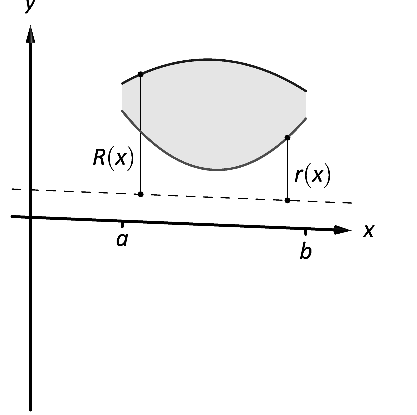
\includegraphics[width=0.35\textwidth]{fig_int_app_13a}}
\qquad
\subfigure[\label{fig_int_app_13b}]{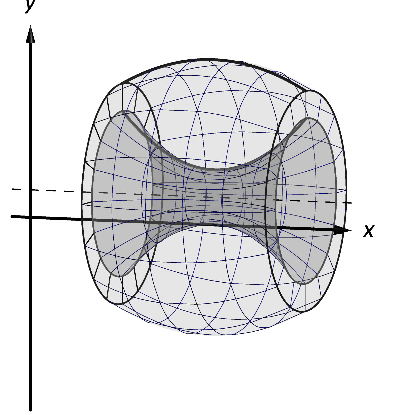
\includegraphics[width=0.35\textwidth]{fig_int_app_13b} }
\qquad
\subfigure[\label{fig_int_app_13c}]{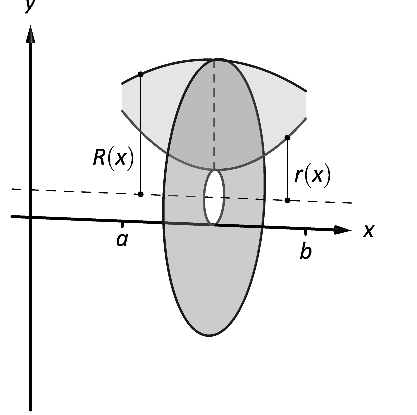
\includegraphics[width=0.35\textwidth]{fig_int_app_13c} }
\caption{Establishing the washer method.}
\end{figure}


Let a region bounded by $y=f(x)$, $y=g(x)$, $x=a$ and $x=b$ be rotated about a horizontal axis that does not intersect the region, forming a solid. Each cross section at $x$ will be a washer with outside radius $R(x)$ and inside radius $r(x)$. The volume of the solid is
\index{integration!washer method}\index{washer method}
\begin{equation}
V = \pi\int\limits_a^b \Big(R(x)^2-r(x)^2\Big)\ dx.
\label{idea:washermethod}
\end{equation}

Obviously, the disk method is just a special case of the washer method with an inside radius of $r(x)=0$.	


\begin{example}\label{ex_wash1}
Find the volume of the solid formed by rotating the region bounded by $y=x^2-2x+2$ and \linebreak $y=2x-1$ about the $x$-axis.

\xhrulefill{gray}{2.5pt}Solution \xhrulefill{gray}{2.5pt}

A sketch of the region will help, as given in Figure \ref{fig_int_app_10a}. Rotating about the $x$-axis will produce cross sections in the shape of washers, as shown in Figure \ref{fig_int_app_14b}; the complete solid is shown in Figure~\ref{fig_int_app_14c}. The outside radius of this washer is $R(x) = 2x-1$; the inside radius is $r(x) = x^2-2x+2$. As the region is bounded from $x=1$ to $x=3$, we integrate as follows to compute the volume.
\begin{align*}
V &= \pi\int\limits_1^3 \Big((2x-1)^2-(x^2-2x+2)^2\Big)\ dx \\[0.2cm]
		&= \pi\int\limits_1^3 \big(-x^4+4x^3-4x^2+4x-3\big)\ dx \\[0.2cm]
		&= \pi\Big[-\frac{1}{5}x^5+x^4-\frac43x^3+2x^2-3x\Big]\Big|_1^3 \\[0.2cm]
		&=\frac{104}{15}\pi\text{ units}^3 \approx 21.78\ \text{units}^3.
\end{align*}	



\end{example}

\begin{figure}[t]
\centering
%\raisebox{0.5cm}{
\subfigure[\label{fig_int_app_14a}]{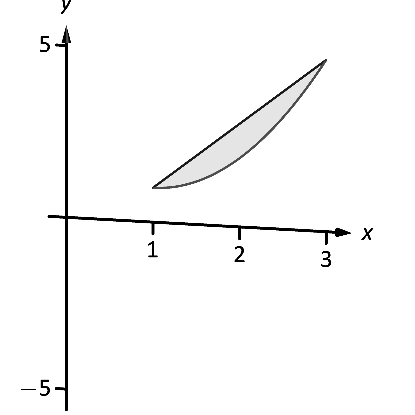
\includegraphics[width=0.35\textwidth]{fig_int_app_14a}}
\qquad
\subfigure[\label{fig_int_app_14b}]{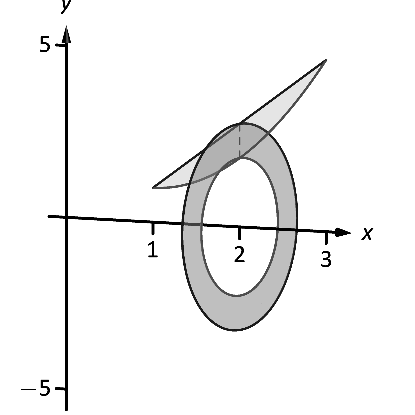
\includegraphics[width=0.35\textwidth]{fig_int_app_14b} }
\qquad
\subfigure[\label{fig_int_app_14c}]{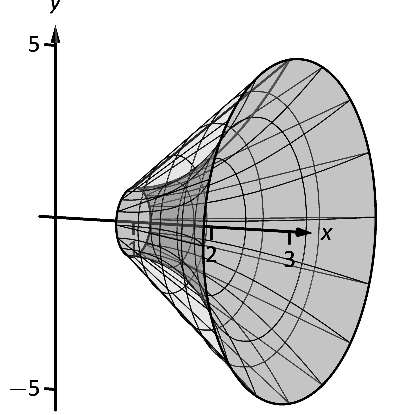
\includegraphics[width=0.35\textwidth]{fig_int_app_14c} }
\caption{Sketching the differential element and solid in Example \ref{ex_wash1}.}
\end{figure}


When rotating about a vertical axis, the outside and inside radius functions must be functions of $y$.\\

\begin{example}\label{ex_wash2}
Find the volume of the solid formed by rotating the triangular region with vertices at $(1,1)$, $(2,1)$ and $(2,3)$ about the $y$-axis.

\xhrulefill{gray}{2.5pt}Solution \xhrulefill{gray}{2.5pt}

The triangular region is sketched in Figure \ref{fig_int_app_15a}; the differential element is sketched in  Figure \ref{fig_int_app_15b} and the full solid is drawn in  Figure \ref{fig_int_app_15c}. They help us establish the outside and inside radii. Since the axis of rotation is vertical, each radius is a function of $y$. 

The outside radius $R(y)$ is formed by the line connecting $(2,1)$ and $(2,3)$; it is a constant function, because $R(y)=2$. The inside radius is formed by the line connecting $(1,1)$ and $(2,3)$. The equation of this line is $y=2x-1$, but we need to refer to it as a function of $y$. Solving for $x$ gives $r(y) = \frac12(y+1)$. 

We integrate over the $y$-bounds of $y=1$ to $y=3$. Thus the volume is

\allowdisplaybreaks
\begin{align*}
V 	&=	\pi\int\limits_1^3\left(2^2 - \left(\frac12(y+1)\right)^2\right)\ dy \\[0.2cm]
		&=	\pi\int\limits_1^3\Big(-\frac14y^2-\frac12y+\frac{15}4\Big)\ dy \\[0.2cm]
		&= 	\pi\Big[-\frac1{12}y^3-\frac14y^2+\frac{15}4y\Big]\Big|_1^3\\[0.2cm]
		&= \frac{10}3\pi\text{units}^3 \approx 10.47\ \text{units}^3.
\end{align*}




\end{example}
\begin{figure}[t]
\centering
%\raisebox{0.5cm}{
\subfigure[\label{fig_int_app_15a}]{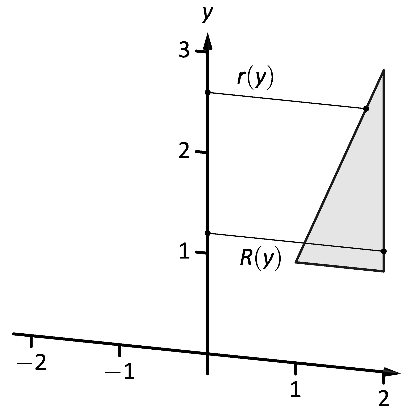
\includegraphics[width=0.35\textwidth]{fig_int_app_15a}}
\qquad
\subfigure[\label{fig_int_app_15b}]{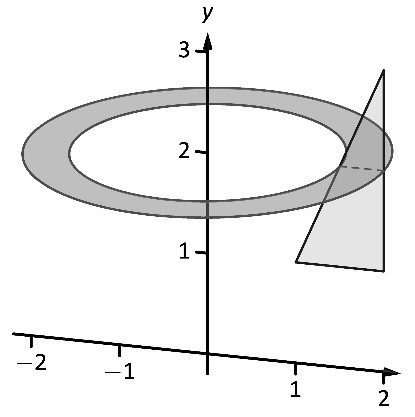
\includegraphics[width=0.35\textwidth]{fig_int_app_15b} }
\qquad
\subfigure[\label{fig_int_app_15c}]{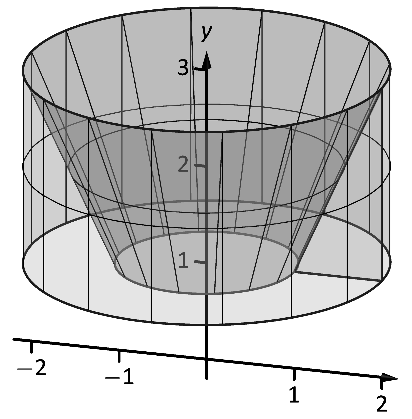
\includegraphics[width=0.35\textwidth]{fig_int_app_15c} }
\caption{Sketching the differential element and solid in Example \ref{ex_wash2}.}
\end{figure}

The ultimate goal of this section is not to compute volumes of solids. That can be useful, but what is more useful is the understanding of this basic principle of integral calculus: to find the exact value of some quantity, 
\begin{itemize}
	\item we start with an approximation (in this section, slice the solid and approximate the volume of each slice), 
	\item then make the approximation better by refining our original approximation (i.e., use more slices), 
	\item	then use limits to establish a definite integral which gives the exact value.
\end{itemize}

We practice this principle in the next section where we find volumes by slicing solids in a different way.

\section{The shell method}\label{sec:shell_method}
This section develops another method of computing volume, the \textbf{shell method.} Instead of slicing the solid perpendicular to the axis of rotation creating cross-sections, we now slice it parallel to the axis of rotation, creating shells.

\checkoddpage
\marginpar{\ifoddpage\hspace*{-1.5cm}\else\hspace*{0.25cm}\fi
\includegraphics[width=0.075\textwidth]{youtube}\\
\ifoddpage\hspace*{-1.75cm}\else\hspace*{0.1cm}\fi
\qrcode[height=1.75cm]{https://youtu.be/Thvc2s9aUP4}
%\includegraphics[width=0.1\textwidth]{schil}
}
Consider Figure \ref{fig_int_app_16a}, where the region is rotated about the $y$-axis forming the solid shown in  Figure \ref{fig_int_app_16b}. A small slice of the region is drawn in  Figure \ref{fig_int_app_16a}, parallel to the axis of rotation. When the region is rotated, this thin slice forms a cylindrical shell, as pictured in Figure \ref{fig_int_app_16c}. The previous section approximated a solid with lots of thin disks (or washers); we now approximate a solid with many thin cylindrical shells. 

\begin{figure}[h]
\centering
%\raisebox{0.5cm}{
\subfigure[\label{fig_int_app_16a}]{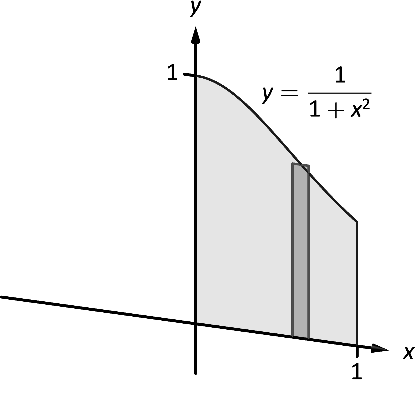
\includegraphics[width=0.35\textwidth]{fig_int_app_16a}}
\qquad
\subfigure[\label{fig_int_app_16b}]{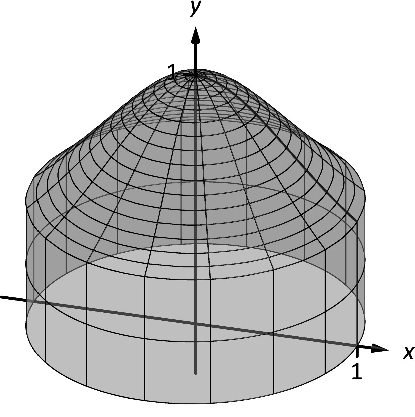
\includegraphics[width=0.35\textwidth]{fig_int_app_16b} }
\qquad
\subfigure[\label{fig_int_app_16c}]{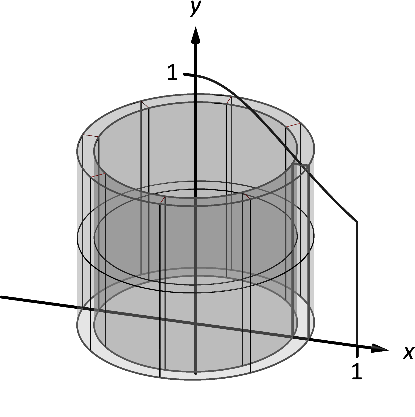
\includegraphics[width=0.35\textwidth]{fig_int_app_16c} }
\caption{The shell method.}
\end{figure}

To compute the volume of one shell, first consider the paper label on a soup can with radius $r$ and height $h$. What is the area of this label? A simple way of determining this is to cut the label and lay it out flat, forming a rectangle with height $h$ and length $2\pi r$. Thus the area is $A = 2\pi rh$; see Figure \ref{fig_int_app_17a}.
Do a similar process with a cylindrical shell, with height $h$, thickness $\Delta x$, and approximate radius $r$. Cutting the shell and laying it flat forms a rectangular solid with length $2\pi r$, height $h$ and depth $\dx$. Thus the volume is $V \approx 2\pi rh\dx$; see Figure \ref{fig_int_app_17b}. We say approximately since our radius was an approximation.


\begin{figure}[h]
\centering
%\raisebox{0.5cm}{
\subfigure[\label{fig_int_app_17a}]{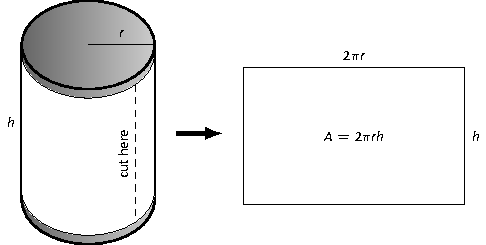
\includegraphics[width=0.45\textwidth]{fig_int_app_17a}}
\qquad
\subfigure[\label{fig_int_app_17b}]{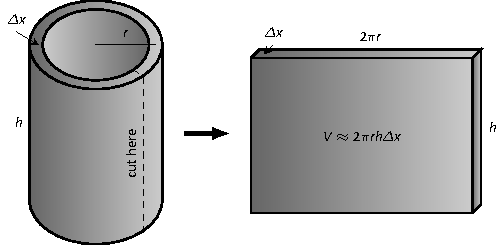
\includegraphics[width=0.45\textwidth]{fig_int_app_17b} }
\caption{Determining the volume of a thin cylindrical shell.}
\end{figure}



%\enlargethispage{2\baselineskip}
By breaking the solid into $n$ cylindrical shells, we can approximate the volume of the solid as
$$V \approx \sum_{i=1}^n 2\pi r_ih_i\dx_i,$$ where $r_i$, $h_i$ and $\dx_i$ are the radius, height and thickness of the $i\,^\text{th}$ shell, respectively. 
This is a Riemann sum. Taking a limit as the thickness of the shells approaches 0 leads to a definite integral.  So we arrive at the following. 

Let a solid be formed by revolving a region $R$, bounded by $x=a$ and $x=b$, about a vertical axis. Let $r(x)$ represent the distance from the axis of rotation to $x$ (i.e., the radius of a sample shell) and let $h(x)$ represent the height of the solid at $x$ (i.e., the height of the shell). The volume of the solid is 
\index{integration!Shell Method}\index{Shell Method}
\begin{equation}
V = 2\pi\int\limits_a^b r(x)h(x)\ dx.
\end{equation}

There are two special cases:
	\begin{enumerate}
	\item		When the region $R$ is bounded above by $y=f(x)$ and below by $y=g(x)$, then $h(x) = f(x)-g(x)$.
	\item		When the axis of rotation is the $y$-axis (i.e., $x=0$) then $r(x) = x$.
	\end{enumerate}
	
Let us practice using this method.

\begin{example}\label{ex_shell1}
Find the volume of the solid formed by rotating the region bounded by $y=0$, $y=1/(1+x^2)$, $x=0$ and $x=1$ about the $y$-axis.

\xhrulefill{gray}{2.5pt}Solution \xhrulefill{gray}{2.5pt}

This is the region used to introduce the shell method in Figure \ref{fig_int_app_16a}, but is sketched again in Figure \ref{fig_int_app_18} for closer reference. A line is drawn in the region parallel to the axis of rotation representing a shell that will be carved out as the region is rotated about the $y$-axis. This is the differential element.

\begin{figure}[H]
	\begin{center}
			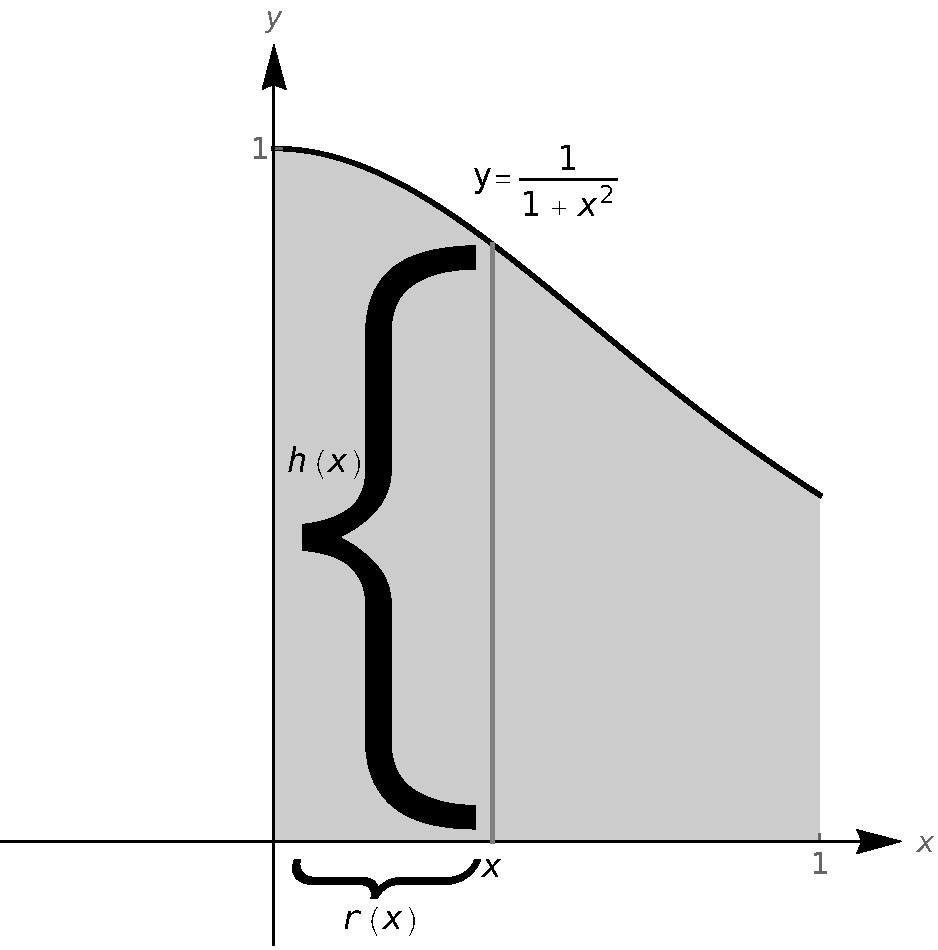
\includegraphics[width=0.5\textwidth]{fig_int_app_18}
	\caption{Graphing a region in Example \ref{ex_shell1}.}
	\label{fig_int_app_18}
	\end{center}
\end{figure}

The distance this line is from the axis of rotation determines $r(x)$; as the distance from $x$ to the $y$-axis is $x$, we have $r(x)=x$. The height of this line determines $h(x)$; the top of the line is at $y=1/(1+x^2)$, whereas the bottom of the line is at $y=0$. Thus $h(x) = 1/(1+x^2)-0 = 1/(1+x^2)$. The region is bounded from $x=0$ to $x=1$, so the volume is 
\begin{align*}
V 	&= 2\pi\int\limits_0^1 \frac{x}{1+x^2}\ dx.
%\end{align*}
\intertext{This requires substitution. Let $u=1+x^2$, so $du = 2x\ dx$. We also change the bounds: $u(0) = 1$ and $u(1) = 2$. Thus we have:}
%\begin{align*}
		&= \pi\int\limits_1^2 \frac{1}{u}\ du \\[0.2cm]
		&= \pi\ln(u)\Big|_1^2\\[0.2cm]
		&= \pi\ln(2) \approx 2.178 \ \text{units}^3.
\end{align*}
Note that in order to find this volume using the disk method, two integrals would be needed to account for the regions above and below $y=1/2$.
\end{example}


With the shell method, nothing special needs to be accounted for to compute the volume of a solid that has a hole in the middle, as demonstrated next.\\

\begin{example}\label{ex_shell2}
Find the volume of the solid formed by rotating the triangular region determined by the points $(0,1)$, $(1,1)$ and $(1,3)$ about the line $x=3$.

\xhrulefill{gray}{2.5pt}Solution \xhrulefill{gray}{2.5pt}

The region is sketched in Figure \ref{fig_int_app_19a} along with the differential element, a line within the region parallel to the axis of rotation. In  Figure \ref{fig_int_app_19b}, we see the shell traced out by the differential element, and in  Figure \ref{fig_int_app_19c} the whole solid is shown.

\begin{figure}[H]
\centering
%\raisebox{0.5cm}{
\subfigure[\label{fig_int_app_19a}]{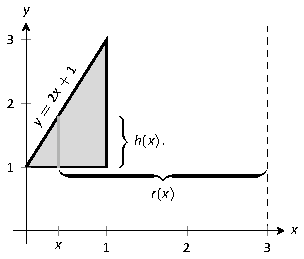
\includegraphics[width=0.35\textwidth]{fig_int_app_19a}}
\qquad
\subfigure[\label{fig_int_app_19b}]{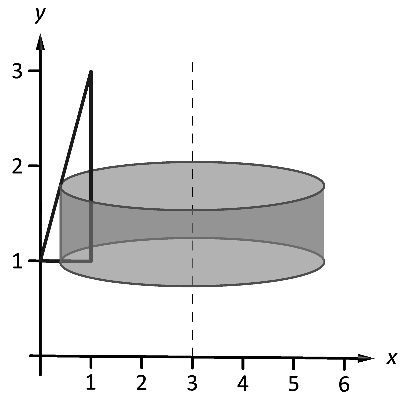
\includegraphics[width=0.35\textwidth]{fig_int_app_19b} }
\qquad
\subfigure[\label{fig_int_app_19c}]{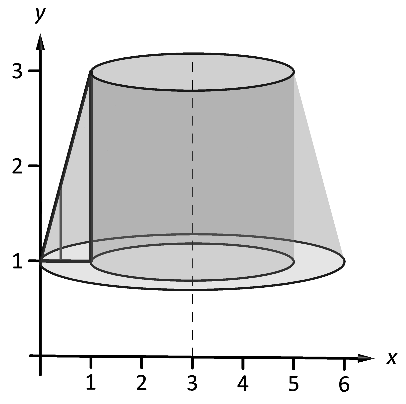
\includegraphics[width=0.35\textwidth]{fig_int_app_19c} }
\caption{Graphing a region in Example \ref{ex_shell2}.}
\end{figure}


The height of the differential element is the distance from $y=1$ to $y=2x+1$, the line that connects the points $(0,1)$ and $(1,3)$. Thus $h(x) = 2x+1-1 = 2x$. The radius of the shell formed by the differential element is the distance from $x$ to $x=3$; that is, it is $r(x)=3-x$. The $x$-bounds of the region are $x=0$ to $x=1$, giving
\allowdisplaybreaks
\begin{align*}
V &=	2\pi\int\limits_0^1 (3-x)(2x)\ dx \\[0.2cm]
	&= 2\pi\int\limits_0^1 \big(6x-2x^2\big)\ dx \\[0.2cm]
	&= 2\pi \Big[3x^2-\frac23x^3 \Big]\Big|_0^1\\
	&= \frac{14}{3}\pi \text{ units}^3\approx 14.66\ \text{units}^3.
\end{align*}




\end{example}

When revolving a region about a horizontal axis, we must consider the radius and height functions in terms of $y$, not $x$.\\

\begin{example}\label{ex_shell3}

Find the volume of the solid formed by rotating the region given in Example \ref{ex_shell2} about the $x$-axis.

\xhrulefill{gray}{2.5pt}Solution \xhrulefill{gray}{2.5pt}

The region is sketched in Figure \ref{fig_int_app_20a} with a sample differential element. In Figure \ref{fig_int_app_20b} the shell formed by the differential element is drawn, and the solid is sketched in Figure \ref{fig_int_app_20c}. 


\begin{figure}[H]
\centering
%\raisebox{0.5cm}{
\subfigure[\label{fig_int_app_20a}]{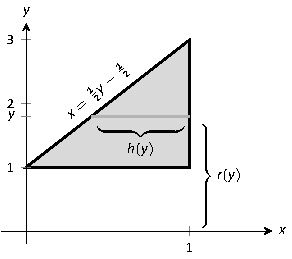
\includegraphics[width=0.35\textwidth]{fig_int_app_20a}}
\qquad
\subfigure[\label{fig_int_app_20b}]{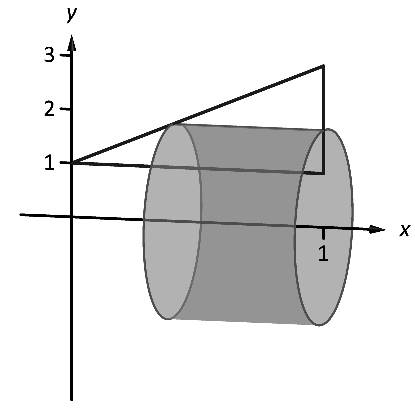
\includegraphics[width=0.35\textwidth]{fig_int_app_20b} }
\qquad
\subfigure[\label{fig_int_app_20c}]{\includegraphics[width=0.35\textwidth]{fig_int_app_20c} }
\caption{Graphing a region in Example \ref{ex_shell3}.}
\end{figure}


The height of the differential element is an $x$-distance, between $x=y/2-1/2$ and $x=1$. Thus $$h(y) = 1-\left(\frac12y-\frac12\right) = -\frac12y+\frac32.$$ The radius is the distance from $y$ to the $x$-axis, so $r(y) =y$. The $y$ bounds of the region are $y=1$ and $y=3$, leading to the integral

\allowdisplaybreaks
\begin{align*}
V &= 2\pi\int\limits_1^3\left[y\left(-\frac12y+\frac32\right)\right]\ dy \\[0.2cm]
	&= 2\pi\int\limits_1^3\left[-\frac12y^2+\frac32y\right]\ dy \\[0.2cm]
  &= 2\pi\Big[-\frac16y^3+\frac34y^2\Big]\Bigg|_1^3 \\[0.2cm]
	&= 2\pi\left[\frac94-\frac7{12}\right]\\[0.2cm]
	&=	\frac{10}{3}\pi  \text{ units}^3 \approx 10.472\, \text{units}^3.
\end{align*}




\end{example}


We end this section with a table summarizing the usage of the washer and shell Methods.
\begin{center}
\begin{tabular}{c|c|c}
 		& Washer method & Shell method\\\hline\hline\\
 Horizontal axis  & $\ds \pi\int\limits_a^b \big(R(x)^2-r(x)^2\big)\ dx$ & $\ds 2\pi\int\limits_c^d r(y)h(y)\ dy$ \\\hline\\
 Vertical axis &  $\ds\pi \int\limits_c^d\big(R(y)^2-r(y)^2\big)\ dy$ & $\ds 2\pi\int\limits_a^b r(x)h(x)\ dx$
 \end{tabular}
\end{center}

In this section, we approximate the volume of a solid by cutting it into thin cylindrical shells. By summing up the volumes of each shell, we get an approximation of the volume. By taking a limit as the number of equally spaced shells goes to infinity, our summation can be evaluated as a definite integral, giving the exact value.

We use this same principle again in the next section, where we find the length of curves in the plane.



\section{Arc length}
\label{sec:arc_length}
\subsection{Rectangular coordinates}
In this section, we address the question: Given a curve, what is its length? This is often referred to as \textbf{arc length} (\textit{booglengte}). \index[aut]{booglengte}\index{arc length}

Consider the graph of $y=\sin(x)$ on $[0,\pi]$ given in Figure \ref{fig_int_app_21a}. How long is this curve? That is, if we were to use a piece of string to exactly match the shape of this curve, how long would the string be?

As we have done in the past, we start by approximating; later, we will refine our answer using limits to get an exact solution.

The length of straight--line segments is easy to compute using the distance formula. We can approximate the length of the given curve by approximating the curve with straight lines and measuring their lengths. 

\begin{figure}
\centering
%\raisebox{0.5cm}{
\subfigure[\label{fig_int_app_21a}]{\includegraphics[width=0.35\textwidth]{fig_int_app_21a}}
\qquad
\subfigure[\label{fig_int_app_21b}]{\includegraphics[width=0.35\textwidth]{fig_int_app_21b} }
\caption{Graphing $y=\sin(x)$ on $[0,\pi]$ (a) and approximating the curve with line segments (b).}
\end{figure}

In Figure \ref{fig_int_app_21b}, the curve $y=\sin(x)$ has been approximated with 4 line segments, i.e.\ the interval $[0,\pi]$ has been divided into 4 equally--lengthed subintervals. It is clear that these four line segments approximate $y=\sin(x)$ very well on the first and last subinterval, though not so well in the middle. Regardless, the sum of the lengths of the line segments is $3.79$, so we approximate the arc length of $y=\sin(x)$ on $[0,\pi]$ to be $3.79$. 


In general,  we can approximate the arc length of $y=f(x)$ on $[a,b]$ in the following manner. Let $a=x_1 < x_2 < \ldots < x_n< x_{n+1}=b$ be a partition of $[a,b]$ into $n$ subintervals. Let $\dx_i$ represent the length of the $i\,^\text{th}$ subinterval $[x_i,x_{i+1}]$. Figure \ref{fig_int_app_22} zooms in on the $i\,^\text{th}$ subinterval where $y=f(x)$ is approximated by a straight line segment. The dashed lines show that we can view this line segment as the hypotenuse of a right triangle whose sides have length $\dx_i$ and $\dy_i$. Using the Pythagorean theorem, the length of this line segment is
$\ds \sqrt{\dx_i^2 + \Delta y_i^2}.$ Summing over all subintervals gives an arc length approximation
$$L \approx \sum_{i=1}^n \sqrt{\dx_i^2 + \Delta y_i^2}.$$


\begin{figure}
	\begin{center}
			\includegraphics[width=0.5\textwidth]{fig_int_app_22}
	\caption{Zooming in on the $i\,^\text{th}$ subinterval $[x_i,x_{i+1}$] of a partition of $[a,b]$.}
	\label{fig_int_app_22}
	\end{center}
\end{figure}


As shown here, this is not a Riemann sum. While we could conclude that taking a limit as the subinterval length goes to zero gives the exact arc length, we would not be able to compute the answer with a definite integral. We need first to do a little algebra.

In the above expression factor out a $\dx_i^2$ term:
\begin{align*}
\sum_{i=1}^n \sqrt{\dx_i^2 + \Delta y_i^2} &= \sum_{i=1}^n \sqrt{\dx_i^2\left(1 + \frac{\Delta y_i^2}{\dx_i^2}\right)}.\\
\intertext{Now pull the $\dx_i^2$ term out of the square root:}%\\
		\sum_{i=1}^n \sqrt{\dx_i^2 + \Delta y_i^2} &= \sum_{i=1}^n\sqrt{1 + \frac{\Delta y_i^2}{\dx_i^2}}\ \dx_i.\\
\intertext{This is nearly a Riemann sum. Consider the $\Delta y_i^2/\dx_i^2$ term. The expression $\Delta y_i/\dx_i$ measures the (change in $y$)/(change in $x$) of $f$ on the $i\,^\text{th}$ subinterval. The mean value theorem of differentiation (Theorem \ref{thm:mvt}) states that there is a $c_i$ in the $i\,^\text{th}$ subinterval where $\fp(c_i) = \Delta y_i/\dx_i$. Thus we can rewrite our above expression as:} 
			\sum_{i=1}^n \sqrt{\dx_i^2 + \Delta y_i^2} &= \sum_{i=1}^n\sqrt{1+\fp(c_i)^2}\ \dx_i.\\
\intertext{This is a Riemann sum. As long as \fp\ is continuous, we can invoke Theorem \ref{thm:riemann_sum} and conclude }%\\
		L &= \int\limits_a^b\sqrt{1+\fp(x)^2}\ dx.
\end{align*}




This result is summarized in the following theorem. 

\begin{theorem}[Arc length]\label{thm:arclength}
Let $f$ be differentiable on $[a,b]$, where $\fp$ is also continuous on $[a,b]$. Then the arc length of $f$ from $x=a$ to $x=b$ is
\index{integration!arc length}\index{arc length}\index[aut]{booglengte}\index[aut]{integratie ! booglengte}
\begin{equation}
L = \int\limits_a^b \sqrt{1+\fp(x)^2}\ dx.
\label{eq_arclength}
\end{equation}
\end{theorem}

The theorem also requires that $\fp$ is continuous on $[a,b]$; while examples are arcane, it is possible for $f$ to be differentiable yet $\fp$ is not continuous.

As the integrand contains a square root, it is often difficult to use Equation~\eqref{eq_arclength} to find the length exactly. When exact answers are difficult to come by, we resort to using numerical methods. 


\begin{example}\label{ex_arc1}
Find the arc length of $f(x) = x^{3/2}$ from $x=0$ to $x=4$. 

\xhrulefill{gray}{2.5pt}Solution \xhrulefill{gray}{2.5pt}

We find $\fp(x)= 3x^{1/2}/2$; note that on $[0,4]$, $f$ is differentiable  and $\fp$ is also continuous. Using Equation~\eqref{eq_arclength}, we find the arc length $L$ as
\allowdisplaybreaks
\begin{align*}
	L &=	\int\limits_0^4 \sqrt{1+\left(\frac32x^{1/2}\right)^2}\ dx \\[0.2cm]
		&=	\int\limits_0^4 \sqrt{1+\frac94x} \ dx \\[0.2cm]
		&=  \frac23\cdot\frac49\cdot\left(1+\frac94x\right)^{3/2}\Big|_0^4 \\[0.2cm]
		&=\frac{8}{27}\left(10^{3/2}-1\right) \approx 9.07 \text{units}.
\end{align*}

	A graph of $f$ is given in Figure \ref{fig_int_app_23}.
	
	
	\begin{figure}[H]
	\begin{center}
			\includegraphics[width=0.4\textwidth]{fig_int_app_23}
	\caption{A graph of $f(x) = x^{3/2}$ from Example \ref{ex_arc1}.}
	\label{fig_int_app_23}
	\end{center}
\end{figure}

\end{example}


We conclude with one example where it is not possible to find an exact answer. 

\begin{example}\label{ex_arc3}
Find the length of the sine curve from $x=0$ to $x=\pi$.

\xhrulefill{gray}{2.5pt}Solution \xhrulefill{gray}{2.5pt}


The setup is straightforward: $f(x) = \sin(x)$ and $\fp(x) = \cos(x)$. Thus 
$$L = \int\limits_0^\pi \sqrt{1+\cos^2(x)}\ dx.$$
This integral cannot be evaluated in terms of elementary functions so we have to approximate it with one of the methods studied in Chapter~\ref{chap_int}. Doing this leads us to  $L\approx 3.8202$.  
\end{example}

\subsection{Parametric and polar equations}

When we are faced with a curve described by parametric equations, we can convert Equation~\eqref{eq_arclength} to such a context.  Letting $x=f(t)$ and $y=g(t)$, we know that $dy/dx = g'(t)/\fp(t)$. It will also be useful to calculate the differential of $x$: 
$$dx = \fp(t)dt \qquad \Rightarrow \qquad dt = \frac{1}{\fp(t)}\,dx.$$
Starting with the arc length formula given by equation~\eqref{eq_arclength}, consider:
\begin{align}
L &= \int\limits_a^b\sqrt{1+\left(\frac{dy}{dx}\right)^2}\ dx\nonumber\\[0.2cm]
		&= \int\limits_a^b \sqrt{1+\frac{g'(t)^2}{\fp(t)^2}}\ dx\nonumber. \\
		&= \int\limits_a^b \sqrt{\fp(t)^2+g'(t)^2}\underbrace{\frac1{\fp(t)}\ dx}_{=dt}\nonumber\\
		&= \int\limits_{t_1}^{t_2} \sqrt{\fp(t)^2+g'(t)^2}\ dt.\nonumber\label{thm:arc_length_parametric}\\
\end{align}
Note the new bounds. They are found by solving $a= f(t)$ and $b=f(t)$ for $t$, and subsequently choosing $t_1$ such that $t_1=\min(t_a,t_b)$, where $t_a$ and $t_b$ are the solutions of  $a= f(t)$ and $b=f(t)$, respectively. Likewise, $t_2$ should be chosen such that $t_2=\max(t_a,t_b)$.

\begin{example}\label{ex_parcalc6}
Find the arc length of the circle parametrized by $x=3\cos(t)$, $y=3\sin(t)$ on $[0,3\pi/2]$. 

\xhrulefill{gray}{2.5pt}Solution \xhrulefill{gray}{2.5pt}

By direct application of Equation~\eqref{thm:arc_length_parametric}, we have
\begin{align*}
L &= \ds\int\limits_0^{3\pi/2} \sqrt{(-3\sin(t))^2 +(3\cos(t))^2} \ dt.\\
\intertext{Then apply the Pythagorean theorem:}
	&= \ds\int\limits_0^{3\pi/2} 3 \ dt= \dfrac{9\pi}{2}\,.
	\end{align*}
	
This should make sense; we know from geometry that the circumference of a circle with radius 3 is $6\pi$; since we are finding the arc length of $3/4$ of a circle, the arc length is $3/4\cdot 6\pi = 9\pi/2$.
\end{example}

As mentioned above, care should be taken when setting the limits of integration for curves defined by means of parametric equations.

\begin{example}\label{ex_parcalc6b}
Find the arc length of the astroid parametrized by $x=c\cos^3(t)$, $y=c\sin^3(t)$ (Figure~\ref{fig_int_app_24}). 


	\begin{figure}[H]
	\begin{center}
			\includegraphics[width=0.4\textwidth]{fig_int_app_24}
	\caption{A graph of the astroid from Example \ref{ex_parcalc6b}.}
	\label{fig_int_app_24}
	\end{center}
\end{figure}

\pagebreak
\xhrulefill{gray}{2.5pt}Solution \xhrulefill{gray}{2.5pt}

By direct application of Equation~\eqref{thm:arc_length_parametric}, we have
\begin{align*}
L &= \ds\int\limits_{t_1}^{t_2} \sqrt{\left(-3c\cos^2(t)\sin(t)\right)^2 +\left(3c\sin^2(t)\cos(t)\right)^2} \ dt\\[0.2cm]
&=\ds\int\limits_{t_1}^{t_2} 3c\sqrt{\sin^2(t)\cos^2(t)\left(\sin^2(t)+\cos^2(t)\right)}\ dt\\[0.2cm]
&=\ds\int\limits_{t_1}^{t_2} \left|3c\sin(t)\cos(t)\right|\ dt\\[0.2cm]
&=\ds\int\limits_{t_1}^{t_2}  \dfrac{3c}{2}\left|\sin(2t)\right|.
	\end{align*}
To find the limits of integration, we note that the arc length we are looking for is four times the length of one arc of the astroid. For what concerns the arc in the first quadrant, we would, when working with cartesian coordinates, vary $x$ from $a=0$ to $b=c$,  where $t$ is $\pi/2$ and $0$, respectively. So, when integrating with respect to $t$ the lower limit of integration should become $t_1=0$ and the upper limit $t_2=\pi/2$. Taking into account these details, we get the following
$$
L =\ds4\int\limits_{0}^{\pi/2}  \dfrac{3c}{2}\sin(2t)=6c.
$$
	
\end{example}


As we have already considered the arc length of curves defined by rectangular and parametric equations, we now consider it as well in the context of polar equations. Recall that the arc length $L$ of the graph defined by the parametric equations $x=f(t)$, $y=g(t)$ on $[a,b]$ is
\index{arc length}
\begin{equation}L = \ds\int\limits_a^b \sqrt{\fp(t)^2 + g'(t)^2}\ dt = \ds\int\limits_a^b \sqrt{x'(t)^2+y'(t)^2}\ dt.\label{eq:polar_arclength}\end{equation}

Now consider the polar function $r=f(\theta)$. We again use the identities $x=f(\theta)\cos(\theta)$ and $y=f(\theta)\sin(\theta)$ to create parametric equations based on the polar function. We compute $x'(\theta)$ and $y'(\theta)$ as done before when computing $\frac{dy}{dx}$, then apply Equation \eqref{eq:polar_arclength}.

The expression $x'(\theta)^2+y'(\theta)^2$ can be simplified a great deal; we leave this as an exercise and state that $$x'(\theta)^2+y'(\theta)^2 = \fp(\theta)^2+f(\theta)^2.$$ This leads us to the  arc length formula.

So, let  $r=f(\theta)$ be a polar function with $\fp$ continuous on $[\alpha,\beta]$, on which the graph traces itself only once. The arc length $L$ of the graph on $[\alpha,\beta]$ is
\begin{equation}
L = \ds\int\limits_\alpha^\beta \sqrt{\fp(\theta)^2+f(\theta)^2}\ d\theta = \ds\int\limits_\alpha^\beta\sqrt{(r\,')^2+ r^2}\ d\theta.
\label{thm:polar_arclength}
\end{equation}

Again, care should be taken when setting the limits of integration for curves defined by means of polar equations.


\section{Surface area}
\label{sec:mantelopp}
\subsection{Rectangular coordinates}
\checkoddpage
\marginpar{\ifoddpage\hspace*{-1.5cm}\else\hspace*{0.25cm}\fi\includegraphics[width=0.075\textwidth]{youtube}\\
\ifoddpage\hspace*{-1.75cm}\else\hspace*{0.1cm}\fi
\qrcode[height=1.75cm]{https://youtu.be/99amc1aaP0E}
%\includegraphics[width=0.1\textwidth]{surface_area}
}
We have already seen how a curve $y=f(x)$ on $[a,b]$ can be revolved about an axis to form a solid. Instead of computing its volume, we now consider its surface area.

We begin as we have in the previous sections: we partition the interval $[a,b]$ with $n$ subintervals, where the $i\,^{\text{th}}$ subinterval is $[x_i,x_{i+1}]$. On each subinterval, we can approximate the curve $y=f(x)$ with a straight line that connects $f(x_i)$ and $f(x_{i+1})$ as shown in Figure \ref{fig_int_app_25a}. Revolving this line segment about the $x$-axis creates part of a cone (called a frustum of a cone) as shown in Figure \ref{fig_int_app_25b}. The surface area of a frustum of a cone is 
$$2\pi\cdot\text{ length }\cdot\text{average of the two radii $R$ and $r$}.$$


\begin{figure}
\centering
%\raisebox{0.5cm}{
\subfigure[\label{fig_int_app_25a}]{\includegraphics[width=0.3\textwidth]{fig_int_app_25a}}
\qquad
\subfigure[\label{fig_int_app_25b}]{\includegraphics[width=0.3\textwidth]{fig_int_app_25b} }
\caption{Establishing the formula for surface area.}
\end{figure}

The length is given by $L_i$. More precisely, we use the material just covered by arc length to state that $$L\approx \sqrt{1+\fp(c_i)^2}\dx_i$$ for some $c_i$ in the $i\,^\text{th}$ subinterval. The radii are just the function evaluated at the endpoints of the interval. That is, $$R_i = f(x_{i+1})\quad \text{and}\quad r_i = f(x_i).$$

Thus the surface area of this sample frustum of the cone is approximately 
$$2\pi\frac{f(x_i)+f(x_{i+1})}2\sqrt{1+\fp(c_i)^2}\dx_i.$$

Since $f$ is a continuous function, the intermediate value theorem states there is some $d_i$ in $[x_i,x_{i+1}]$ such that $ f(d_i) = \frac{f(x_i)+f(x_{i+1})}2$; we can use this to rewrite the above equation as
$$2\pi f(d_i)\sqrt{1+\fp(c_i)^2}\dx_i.$$
Summing over all the subintervals we get the total surface area to be approximately 
$$SA\approx \sum_{i=1}^n 2\pi f(d_i)\sqrt{1+\fp(c_i)^2}\dx_i,$$
which is a Riemann sum. Taking the limit as the subinterval lengths go to zero gives us the exact surface area, given in the following theorem.

\begin{theorem}[Surface area of a solid of revolution using rectangular coordinates]\label{thm:surface_area}
Let $f$ be differentiable on  $[a,b]$, where $\fp$ is also continuous on $[a,b]$. \index{integration!surface area}\index{surface area}\index[aut]{manteloppervlakte}\index[aut]{integratie ! manteloppervlakte}
	\begin{enumerate}
	\item	The surface area of the solid formed by revolving the graph of $y=f(x)$, where $f(x)\geq0$, about the $x$-axis is
	$$SA = 2\pi\int\limits_a^b f(x)\sqrt{1+\fp(x)^2}\ dx.$$
	\item	The surface area of the solid formed by revolving the graph of $y=f(x)$ about the $y$-axis, where $a,b\geq0$, is
	$$SA = 2\pi\int\limits_a^b x\sqrt{1+\fp(x)^2}\ dx.$$
	\end{enumerate}
\end{theorem}

When revolving $y=f(x)$ about the $y$-axis, the radii of the resulting frustum are $x_i$ and $x_{i+1}$; their average value is simply the midpoint of the interval. In the limit, this midpoint is just $x$. This gives the second part of Theorem \ref{thm:surface_area}.

\ifanalysis

\begin{example}\label{ex_sa1}
Find the surface area of the solid formed by revolving $y=\sin(x)$ on $[0,\pi]$ about the $x$-axis, as shown in Figure \ref{fig_int_app_26}.

	\begin{figure}[H]
	\begin{center}
			\includegraphics[width=0.5\textwidth]{fig_int_app_26}
	\caption{Revolving $y=\sin (x)$ on $[0,\pi]$ about the $x$-axis.}
	\label{fig_int_app_26}
	\end{center}
\end{figure}


\xhrulefill{gray}{2.5pt}Solution \xhrulefill{gray}{2.5pt}

The setup is relatively straightforward. Using Theorem \ref{thm:surface_area}, we have the surface area $SA$ is:
\begin{align*}
SA  &=	2\pi\int\limits_0^\pi \sin(x)\sqrt{1+\cos^2(x)}\ dx \\
		&=	-2\pi\frac12\left.\left(\arsinh(\cos(x))+\cos(x)\sqrt{1+\cos^2(x)}\right)\right|_0^\pi \\
		&= 2\pi\left(\sqrt{2}+\arsinh(1)\right) \approx 14.42\ \text{units}^2.%\\
		%&\approx 14.42\ \text{units}^2.
\end{align*}
The integration step above is nontrivial uses trigonometric substitution. 

It is interesting to see that the surface area of a solid, whose shape is defined by a trigonometric function, involves both a square root and an inverse hyperbolic trigonometric function.
\end{example}


\begin{example}\label{ex_sa2}
Find the surface area of the solid formed by revolving the curve $y=x^2$ on $[0,1]$ about the $x$-axis and the $y$-axis.
		%\begin{enumerate}
		%\item		the $x$-axis
		%\item		the $y$-axis.
		%\end{enumerate}
		
\xhrulefill{gray}{2.5pt}Solution \xhrulefill{gray}{2.5pt}
		
%\begin{enumerate}
	%\item		
	About the $x$-axis: the integral is straightforward to setup:
	\allowdisplaybreaks
	\begin{align*}
	SA &= 2\pi\int_0^1 x^2\sqrt{1+(2x)^2}\ dx.
	\intertext{Like the integral in Example \ref{ex_sa1}, this requires trigonometric substitution.}
		&= \left.\frac{\pi}{32}\left(2(8x^3+x)\sqrt{1+4x^2}-\arsinh(2x)\right)\right|_0^1\\
		&=\frac{\pi}{32}\left(18\sqrt{5}-\arsinh(2)\right)\\
		&\approx 3.81\ \text{units}^2.
	\end{align*}
	The solid formed by revolving $y=x^2$ about the $x$-axis is graphed in Figure \ref{fig_int_app_27a}.

	%\item	 
	About the $y$-axis: since we are revolving about the $y$-axis, the radius of the solid is not $f(x)$ but rather $x$. Thus the integral to compute the surface area is:
	\begin{align*}
	SA &= 2\pi\int_0^1x\sqrt{1+(2x)^2}\ dx.
		\intertext{This integral can be solved using substitution. Set $u=1+4x^2$; the new bounds are $u=1$ to $u=5$. We then have }
		&=	\frac{\pi}4\int_1^5 \sqrt{u}\ du \\
		&= \frac{\pi}6\left(5\sqrt{5}-1\right)\\
		&\approx 5.33\ \text{units}^2.
	\end{align*}
 The solid formed by revolving $y=x^2$ about the $y$-axis is graphed in Figure \ref{fig_int_app_27b}.	

\begin{figure}[H]
\centering
%\raisebox{0.5cm}{
\subfigure[\label{fig_int_app_27a}]{\includegraphics[width=0.45\textwidth]{fig_int_app_27a}}
\qquad
\subfigure[\label{fig_int_app_27b}]{\includegraphics[width=0.45\textwidth]{fig_int_app_27b} }
\caption{The solids used in Example \ref{ex_sa2}.}
\end{figure}


\end{example}


\fi


We conclude this section with a famous mathematical paradox.
%\clearpage

\begin{example}\label{ex_gabriel}
Consider the solid formed by revolving $y=1/x$ about the $x$-axis on $[1,+\infty[$. Find the volume and surface area of this solid. This shape, as graphed in Figure \ref{fig_int_app_28}, is known as ``Gabriel's Horn'' since it looks like a very long horn that only a supernatural person, such as an angel, could play.


\xhrulefill{gray}{2.5pt}Solution \xhrulefill{gray}{2.5pt}

To compute the volume it is natural to use the disk method. We have:

\allowdisplaybreaks
\begin{align*}
V &= \pi\int\limits_1^{+\infty} \frac{1}{x^2}\ dx \\[0.2cm]
	&= \lim_{b\to+\infty}\pi\int\limits_1^b\frac{1}{x^2}\ dx \\[0.2cm]
	&= \lim_{b\to+\infty} \pi\left(1-\frac1b\right) \\
	&= \pi \ \text{units}^3.
\end{align*}
Gabriel's Horn has a finite volume of $\pi$ cubic units. Since we have already seen that regions with infinite length can have a finite area, this is not too difficult to accept.

	\begin{figure}[H]
	\begin{center}
			\includegraphics[width=0.5\textwidth]{fig_int_app_28}
	\caption{A graph of Gabriel's Horn.}
	\label{fig_int_app_28}
	\end{center}
\end{figure}

\ifanalysis
We now consider its surface area. The integral is straightforward to setup:
\begin{align*}
SA &= 2\pi\int\limits_1^{+\infty} \frac{1}{x}\sqrt{1+\dfrac{1}{x^4}}\ dx.
\intertext{Integrating this expression is not trivial. We can, however, compare it to other improper integrals. Since $1< \sqrt{1+1/x^4} $ on $[1,+\infty[$, we can state that}
2\pi\int\limits_1^{+\infty} \frac{1}{x}\ dx &<2\pi\int\limits_1^{+\infty} \frac{1}{x}\sqrt{1+\dfrac{1}{x^4}}\ dx .
\end{align*}
The improper integral on the left diverges. Since the integral on the right is larger, we conclude it also diverges, meaning Gabriel's Horn has infinite surface area.
\fi 

\ifcalculus
We now consider its surface area. The integral is straightforward to setup:
$$
SA = 2\pi\int\limits_1^{+\infty} \frac{1}{x}\sqrt{1+\dfrac{1}{x^4}}\ dx.
$$
Integrating this expression is not trivial, but it can be shown that this improper integral  diverges, meaning Gabriel's Horn has infinite surface area.
\fi
Hence the paradox: we can fill Gabriel's Horn with a finite amount of paint, but since it has infinite surface area, we can never paint it.
\enlargethispage{3\baselineskip}

\end{example}

\subsection{Parametric and polar equations}
When dealing with a plane curve described by parametric equations, we can adapt the formula found in Theorem \ref{thm:surface_area} in a similar way as done to produce the formula for arc length done before.

%\setboxwidth{100pt}

\begin{theorem}[Surface area of a solid of revolution using parametric equations]\label{thm:surface_area_parametric}
Consider the graph of the parametric equations $x=f(t)$ and $y=g(t)$, where $\fp$ and $g'$ are continuous on an open interval $I$ containing $t_1$ and $t_2$ on which the graph does not cross itself.\index{surface area!solid of revolution}\index{integration!surface area}\index{parametric equations!surface area}
\begin{enumerate}
	\item	The surface area of the solid formed by revolving the graph about the $x$-axis is (where $g(t)\geq 0$ on $[t_1,t_2]$):
	$$SA = 2\pi\int\limits_{t_1}^{t_2} g(t)\sqrt{\fp(t)^2+g'(t)^2}\ dt.$$
	
	\item	The surface area of the solid formed by revolving the graph about the $y$-axis is (where $f(t)\geq 0$ on $[t_1,t_2]$):
	$$SA = 2\pi\int\limits_{t_1}^{t_2} f(t)\sqrt{\fp(t)^2+g'(t)^2}\ dt.$$
	\end{enumerate}
\end{theorem}
	
\begin{example}\label{ex_parcalc8}
Consider the teardrop shape formed by the parametric equations $x=t(t^2-1)$, $y=t^2-1$. Find the surface area if this shape is rotated about the $x$-axis, as shown in Figure \ref{fig_int_app_29}.

	\begin{figure}[H]
	\begin{center}
			\includegraphics[width=0.5\textwidth]{fig_int_app_29}
	\caption{Rotating a teardrop shape about the $x$-axis in Example \ref{ex_parcalc8}.}
	\label{fig_int_app_29}
	\end{center}
\end{figure}

\xhrulefill{gray}{2.5pt}Solution \xhrulefill{gray}{2.5pt}

The teardrop shape is formed between $t=-1$ and $t=1$. Using Theorem \ref{thm:surface_area_parametric}, we see we need for $g(t)\geq 0$ on $[-1,1]$, and this is not the case. To fix this, we simplify replace $g(t)$ with $-g(t)$, which flips the whole graph about the $x$-axis. The surface area is: 
\begin{align*}
SA &= 2\pi\int\limits_{-1}^1 (1-t^2)\sqrt{(3t^2-1)^2+(2t)^2}\ dt\\[0.2cm]
		&=	2\pi\int\limits_{-1}^1 (1-t^2)\sqrt{9t^4-2t^2+1} \ dt.
		\end{align*}
Once again we arrive at an integral that we cannot compute in terms of elementary functions. Using the midpoint rule with $n=20$, we find the area to be approximately $S=9.44$. 
\end{example}

When dealing with polar equations, we may resort to the following theorem to find surface areas of solids of revolution. 

\begin{theorem}[Surface area of a solid of revolution using polar equations]\label{thm:surface_area_polar}
Consider the graph of the polar equation $r=f(\theta)$, where $\fp$ is continuous on  $[\alpha,\beta]$, on which the graph does not cross itself.
\index{integration!surface area}\index[aut]{manteloppervlakte}
	\begin{enumerate}
		\item The surface area of the solid formed by revolving the graph about the initial ray ($\theta=0$) is:
		$$SA = 2\pi\int\limits_\alpha^\beta f(\theta)\sin(\theta)\sqrt{\fp(\theta)^2+f(\theta)^2}\ d\theta.$$
		\item The surface area of the solid formed by revolving the graph about the line $\theta=\pi/2$ is:
		$$SA = 2\pi\int\limits_\alpha^\beta f(\theta)\cos(\theta)\sqrt{\fp(\theta)^2+f(\theta)^2}\ d\theta.$$
	\end{enumerate}
\end{theorem}

\begin{example}\label{ex_polcalc8}
Find the surface area formed by revolving one petal of the rose curve $r=\cos(2\theta)$ about its central axis (see Figure \ref{fig_int_app_30a}).



\xhrulefill{gray}{2.5pt}Solution \xhrulefill{gray}{2.5pt}

We choose, as implied by the figure, to revolve the portion of the curve that lies on $[0,\pi/4]$ about the initial ray. Using Theorem \ref{thm:surface_area_polar} and the fact that $\fp(\theta) = -2\sin(2\theta)$, we have
\begin{align*}
SA &= 2\pi\int\limits_0^{\pi/4} \cos(2\theta)\sin(\theta)\sqrt{\big(-2\sin(2\theta)\big)^2+\big(\cos(2\theta)\big)^2}\ d\theta \\
&\approx 1.36707.
\end{align*}
The integral is another that cannot be evaluated in terms of elementary functions. The midpoint's rule, with $n=4$, approximates the value at $1.37$.


\begin{figure}[H]
\centering
%\raisebox{0.5cm}{
\subfigure[\label{fig_int_app_30a}]{\includegraphics[width=0.45\textwidth]{fig_int_app_30a}}
\qquad
\subfigure[\label{fig_int_app_30b}]{\includegraphics[width=0.45\textwidth]{fig_int_app_30b} }
\caption{Finding the surface area of a rose--curve petal that is revolved about its central axis.}
\end{figure}

\end{example}

\ifanalysis



\section{Work}\label{sec:work}


Work is the scientific term used to describe the action of a force which moves an object. When a constant force $F$ is applied to move an object a distance $d$, the amount of work performed is $W=F\cdot d$. The SI unit of force is the Newton, (kg$\cdot$m/s$^2$), and the SI unit of distance is a meter (m). The fundamental unit of work is one Newton--meter, or a joule (J). That is, applying a force of one Newton for one meter performs one joule of work.

When force is constant, the measurement of work is straightforward. For instance, lifting an object with of force of 200 N for 5 m gives rise $200\cdot 5 = 1000$ J of work. What if the force applied is variable? For instance, imagine a climber pulling a 200 m rope up a vertical face. The rope becomes lighter as more is pulled in, requiring less force and hence the climber performs less work.

In general, let $F(x)$ be a force function on an interval $[a,b]$. We want to measure the amount of work done applying the force $F$ from $x=a$ to $x=b$. We can approximate the amount of work being done by partitioning $[a,b]$ into subintervals $a=x_1<x_2 <\cdots <x_{n+1}=b$ and assuming that $F$ is constant on each subinterval. Let $c_i$ be a value in the $i\,^{\text{th}}$ subinterval $[x_i,x_{i+1}]$. Then the work done on this interval is approximately $W_i\approx F(c_i)(x_{i+1}-x_i) = F(c_i)\dx_i$, a constant force $\times$ the distance over which it is applied. The total work is 
$$ W = \sum_{i=1}^n W_i \approx \sum_{i=1}^n F(c_i)\dx_i.$$
This, of course, is a Riemann sum. Taking a limit as the subinterval lengths go to zero gives an exact value of work which can be evaluated through a definite integral. 


So, if we let $F(x)$ be a continuous function on $[a,b]$ describing the amount of force being applied to an object in the direction of travel from distance $x=a$ to distance $x=b$, then the total work $W$ done on $[a,b]$ is
\index{integration!work}\index{work}\index[aut]{arbeid}
\begin{equation}
W = \int\limits_a^b F(x)\ dx.
\label{idea:work}
\end{equation}

\begin{example}\label{ex_work1}
A 60m climbing rope is hanging over the side of a tall cliff. 

\begin{enumerate}
\item How much work is performed in pulling the rope up to the top, where the rope has a mass of 66g/m? 
\item At what point is exactly half the work performed?
\end{enumerate}
%How much work is performed pulling a 60 m climbing rope up a cliff face, where the rope has a mass of 66 g/m?

\xhrulefill{gray}{2.5pt}Solution \xhrulefill{gray}{2.5pt}

\begin{enumerate}
\item We need to create a force function $F(x)$ on the interval $[0,60]$. To do so, we must first decide what $x$ is measuring: it is the length of the rope still hanging or is it the amount of rope pulled in? As long as we are consistent, either approach is fine. We adopt for this example the convention that $x$ is the amount of rope pulled in. This seems to match intuition better; pulling up the first 10 meters of rope involves $x=0$ to $x=10$ instead of $x=60$ to $x=50$. 

As $x$ is the amount of rope pulled in, the amount of rope still hanging is $60-x$. This length of rope has a mass of 66 g/m, or $0.066$ kg/m. The mass of the rope still hanging is $0.066(60-x)$ kg; multiplying this mass by the acceleration of gravity, 9.8 m/s$^2$, gives our variable force function $$F(x) = (9.8)(0.066)(60-x) = 0.6468(60-x).$$

Thus the total work performed in pulling up the rope is 
$$W = \int\limits_0^{60} 0.6468(60-x)\ dx = 1164.24\ \text{J}.$$

By comparison, consider the work done in lifting the entire rope 60 meters. The rope weighs $60\times 0.066 \times 9.8 = 38.808$ N, so the work applying this force for 60 meters is $60\times 38.808 = 2328.48$ J. This is exactly twice the work calculated before.

\item we know the total work performed is $1164.24$ J. We want to find a height $h$ such that the work in pulling the rope from a height of $x=0$ to a height of $x=h$ is 582.12, half the total work. Thus we want to solve the equation
%\enlargethispage{\baselineskip}
$$\int\limits_0^h 0.6468(60-x)\ dx = 582.12$$ 
for $h$. 
$$
\begin{array}{rrcl}
&\int\limits_0^h 0.6468(60-x)\ dx &=& 582.12 \\[0.2cm]
\Leftrightarrow&\quad\left(38.808x-0.3234x^2\right)\Big|_0^h &=&582.12 \\[0.2cm]
\Leftrightarrow&\quad38.808h-0.3234h^2 &=&582.12 \\[0.2cm]
\Leftrightarrow&\quad-0.3234h^2+38.808h-582.12 &=&0
\end{array}
$$

Apply the quadratic formula:
\[h =17.57 \quad \text{ and } \quad h= 102.43\,. \]
As the rope is only 60m long, the only sensible answer is $h=17.57$. Thus about half the work is done pulling up the first 17.5m the other half of the work is done pulling up the remaining 42.43m. 
\end{enumerate}
\end{example}

	\begin{center}
			\includegraphics[width=0.65\textwidth]{GreatMath_4.jpg}
	\end{center}

 
% Another useful example of the application of integration to compute work comes in the pumping of fluids, often illustrated in the context of emptying a storage tank by pumping the fluid out the top. This situation is different than our previous examples for the forces involved are constant. After all, the force required to move one cubic metre of water  is the same regardless of its location in the tank. What is variable is the distance that cubic foot of water has to travel; water closer to the top travels less distance than water at the bottom, producing less work.


% \begin{example}\label{ex_pump1}
% A cylindrical storage tank with a radius of 10 m and a height of 30 m is filled with a fluid, which weighs approximately 62.4 kg/m$^3$. Compute the amount of work performed by pumping the water up to a point 5 metres above the top of the tank.  Figure \ref{fig_int_app_31} which illustrates the  aspects of this problem.

% 	\begin{figure}[H]
% 	\begin{center}
% 			\includegraphics[width=0.5\textwidth]{fig_int_app_31}
% 	\caption{Illustrating a water tank in order to compute the work required to empty it in Example \ref{ex_pump1}.}
% 	\label{fig_int_app_31}
% 	\end{center}
% \end{figure}

% \xhrulefill{gray}{2.5pt}Solution \xhrulefill{gray}{2.5pt}


% We start as we often do: we partition an interval into subintervals. We orient our tank vertically since this makes intuitive sense with the base of the tank at $y=0$. Hence the top of the water is at $y=30$, meaning we are interested in subdividing the $y$-interval $[0,30]$ into $n$ subintervals as 
% $$0 = y_1 < y_2 < \cdots < y_{n+1} = 30.$$
% Consider the work $W_i$ of pumping only the water residing in the $i\,^\text{th}$ subinterval, illustrated in Figure \ref{fig_int_app_31}. The force required to move this water is equal to its weight which we calculate as volume $\times $ density. The volume of water in this subinterval is 
% $V_i = 10^2\pi \Delta y_i$; its density is $62.4$ kg/m$^3$. Thus the required force is $6240\pi\Delta y_i$ N.

% We approximate the distance the force is applied by using any $y$-value contained in the $i\,^\text{th}$ subinterval; for simplicity, we arbitrarily use $y_i$ for now (it will not matter later on). The water will be pumped to a point 5 metres above the top of the tank, that is, to the height of $y=35$ m. Thus the distance the water at height $y_i$ travels is $35-y_i$ m. 

% In all, the approximate work $W_i$ peformed in moving the water in the $i\,^\text{th}$ subinterval to a point 5 metres above the tank is 
% $$W_i \approx 6240\pi\Delta y_i(35-y_i).$$
% To approximate the total work performed in pumping out all the water from the tank, we sum all the work $W_i$ performed in pumping the water from each of the $n$ subintervals of $[0,30]$:
% $$W \approx \sum_{i=1}^n W_i = \sum_{i=1}^n 6240\pi\Delta y_i(35-y_i).$$
% This is a Riemann sum. Taking the limit as the subinterval length goes to 0 gives 
% \begin{align*}
% W 	&=	\int\limits_0^{30} 6240\pi(35-y)\ dy \\[0.2cm]
% 		&=  6240\pi\left(35y-1/2y^2\right)\Big|_0^{30} \\[0.2cm]
% 		&= 	11,762,123 \ \text{Nm}\\[0.2cm]
% 		&\approx  1.176 \times 10^7 \ \text{Nm}.
% \end{align*}
% \end{example}

\fi

\newpage
\section{Exercises}

\renewcommand{\ExerciseListName}{Assignement}

\subsection*{\nameref{sec:ABC}}
%%%%%%%%%%%%%%%%%%%
%Oefening 1
%%%%%%%%%%%%%%%%%%%
\begin{Exercise} Sketch the regions below and find their area.

\Question[difficulty = 1] the area bounded by $y^2=4x$ and $y=2x-4$

\Question[difficulty = 1] the area bounded by $x=4-y^2$ and the $y$-axis

\Question[difficulty = 1] the smallest part within $x^2 + y^2=25$, cut off by $x=3$

\ifcalculus \Question[difficulty = 2] \fi  \ifanalysis \Question[difficulty = 1] \fi the region enclosed between $y=4x-x^2$, $y=4-x$ and the $y$-axis
\ifcalculus \Question[difficulty = 2] \fi \ifanalysis \Question[difficulty = 1] \fi the region enclosed between $y=6x-x^2$ and $y=x^2-2x$

\ifanalysis\Question[difficulty = 1]\fi \ifcalculus\Question[difficulty = 2]\fi the region enclosed between $x^2 + y^2=12$ and $y^2=x$

\ifanalysis\Question[difficulty = 1]\fi \ifcalculus\Question[difficulty = 2]\fi the region enclosed between $y=0$ and $y= \cos^2(x)$ for $x \in [0,2\pi]$

\ifanalysis \Question[difficulty = 1] \fi \ifcalculus\Question[difficulty = 2]\fi the region enclosed between $y=\ln (2x)$ and $y= \ln(x)$ for $x \in [1,e]$ 
\ifanalysis
\Question[difficulty = 1] the region enclosed between $y=\cosh (x)$ and $y= \sinh (x)$ for $x \in [0,1]$  
\fi
\ifanalysis\Question[difficulty = 2]\fi \ifcalculus\Question[difficulty = 3]\fi the region enclosed between $y = \sin (x)$, $x+y+\dfrac{\pi}{2} + 1 = 0$ and the $x$-axis

\end{Exercise}

\setboolean{firstanswerofthechapter}{true}
\begin{Answer}

\Question $A=\ds \int\limits_{-2}^{4} \left( \dfrac{y}{2} + 2 - \dfrac{y^2}{4}  \right)\, dy = 9$ \quad or \quad $A=4 \ds \int\limits_{0}^{1} \sqrt{x} \, dx + \ds \int\limits_{1}^{4} \left( 2\sqrt{x}-2x+4 \right) \, dx=9$

\Question $A =  2 \ds \int\limits_{0}^{2}(4-y^2) \, dy =  \dfrac{32}{3}$ \quad or \quad $A = 2 \ds \int\limits_{0}^{4} \sqrt{4-x} \, dx =  \dfrac{32}{3}$

\Question $A=2 \ds \int\limits_{3}^{5} \sqrt{25-x^2} \, dx = -12 + \dfrac{25 \pi}{2}-25 \arcsin \left( \dfrac{3}{5}  \right) = 25 \arccos \left( \dfrac{3}{5}  \right) -12 $ 

 or \quad $A=2 \ds \int\limits_{0}^{4} \left( \sqrt{25-y^2} -3  \right)\, dy = 25 \arccos \left( \dfrac{3}{5}  \right) -12 $

%\ifcalculus 
\Question $A= \ds \int\limits_{0}^{1}\left(\left(4-x\right) - \left(4x-x^2\right)  \right) \, dx + \ds \int\limits_{1}^{4} \left( \left(4x-x^2 \right) - \left(4-x \right) \right) \, dx= \dfrac{19}{3}$

 This exercise is not suited to use $y$ as variable of integration. 
%\fi 

%\ifcalculus 
\Question $A =\ds \int\limits_{0}^{4}\left(6x-x^2 - \left( x^2-2x \right) \right) \, dx = \ds \int\limits_{0}^{4}\left(8x-2x^2 \right) \, dx = \dfrac{64}{3}$ 

 This exercise is not suited to use $y$ as variable of integration.  
%\fi

\Question $A=2 \ds \int\limits_{0}^{3} \sqrt{x} \, dx + 2 \ds \int\limits_{3}^{2 \sqrt{3}} \sqrt{12-x^2} \, dx = 2 \left( \dfrac{\sqrt{3}}{2} + \pi\right) $

 or \quad $A=2 \ds \int\limits_{0}^{\sqrt{3}} \left( \sqrt{12-y^2} - y^2 \right)\, dy = 2 \left( \dfrac{\sqrt{3}}{2} + \pi\right)$
 
\Question $A=2 \ds \int\limits_{\pi/2}^{3\pi/2} \cos^2(x) \ dx= \pi $ \quad of \quad $A=4 \ds \int\limits_{0}^{1} \arccos \left( \sqrt{y} \right)\ dy= \pi$
	
\Question $A= \ds \int\limits_{1}^{e} \left( \ln(2x) - \ln(x) \right) \ dx = (e-1) \ln(2)$

 or \quad $A= \ds \int\limits_{0}^{\ln(2)} \left( e^{y} - 1 \right)\ dy + \ds \int\limits_{\ln(2)}^{1} \left( e^{y} - \dfrac{e^y}{2} \right) \ dy + \ds \int\limits_{1}^{\ln(2e)} \left( e - \dfrac{e^y}{2} \right)\ dy= (e-1) \ln(2)$

\ifanalysis

\Question $A= \ds \int\limits_{0}^{1} \left( \cosh(x) - \sinh(x) \right) \ dx = 1-\dfrac{1}{e}$

 or \quad $A= \ds \int\limits_{0}^{1} \arsinh(y)\ dy + \ds \int\limits_{1}^{\sinh(1)} \left( \arsinh(y)- \arcosh(y) \right) \ dy + \ds \int\limits_{\sinh(1)}^{\cosh(1)} \left( 1 - \arcosh(y)\right)\ dy= 1-\dfrac{1}{e}$

\fi

\Question $A= \ds \int\limits_{-\pi/2-1}^{-\pi/2} \left( x + \dfrac{\pi}{2} + 1 \right) \, dx + \ds \int\limits_{-\pi/2}^{0} \left(- \sin(x) \right) \, dx = \dfrac{3}{2}$

 or \quad $ A=\ds \int\limits_{-1}^{0} \left( 1+y+  \dfrac{\pi}{2} + \arcsin(y) \right)\, dy= \dfrac{3}{2}$

\end{Answer}
\setboolean{firstanswerofthechapter}{false}

%%%%%%%%%%%%%%%%%%%
%Oefening 2
%%%%%%%%%%%%%%%%%%%
\begin{Exercise} Find the areas of the regions below.
\ifcalculus
\Question[difficulty = 1] a sector of a circle of radius $R$ about an angle $\alpha$
\Question[difficulty = 1] the region enclosed between the parabola $y^2=4a(a-x)$, with $a>0$, and the $y$-axis
\Question[difficulty = 1] the region enclosed between $y=\dfrac{x^2}{2}$, $y = \sqrt{2x}$ and $y = \sqrt{2} x$
\fi
\ifanalysis\Question[difficulty = 1]\fi\ifcalculus\Question[difficulty = 2]\fi the area inside the loop of the curve $\left\{ \begin{array}{l} x = t^2 \\ y = t- \dfrac{t^3}{9}   \end{array}  \right.$

\ifcalculus
\Question[difficulty = 2] The  region enclosed by  the cardioid $r(\theta) = a(1+ \cos(\theta))$
\Question[difficulty = 2] The  region enclosed by one loop of the curve $r(\theta) = 4 \cos(2 \theta) $
\Question[difficulty = 2] the area  region enclosed by  the astroid
\[ \left \{\begin{array}{l}
x = c \cos^3 (t)\\
y = c \sin^3 (t) .
\end{array}\right. \] 
\ifanalysis\Question[difficulty = 2]\fi\ifcalculus\Question[difficulty = 3]\fi The area  region enclosed by  the curve $\left\{\begin{array}{l} x = 3 + \cos(\theta) \\ y = 4 \sin(\theta)   \end{array} \right.$ 
\ifanalysis\Question[difficulty = 2]\fi\ifcalculus\Question[difficulty = 3]\fi the area  region enclosed by  the curve $\left\{ \begin{array}{l} x = 3 \sin(2t) \\ y = 2 \cos(t)  \end{array}  \right.$ 

\Question[difficulty = 2] The region outside the circle $r=2$ and  enclosed by  the cardioid $r = 2 \left( \cos(\theta) + 1 \right)$

\Question[difficulty = 2] The  region enclosed by  the circle $r=2$ and within the cardioid $r = 2 \left( \cos(\theta) - 1 \right)$

\Question[difficulty = 3] the region outside of the curve $r=a$ and   enclosed by  $r(\theta)=2a \sin(3 \theta)$
\Question[difficulty = 3] the common region enclosed by the curves $\sqrt{3} r(\theta)= 1+\sin(\theta)$ en $ r(\theta) = \cos(\theta)$
\fi


\ifanalysis
\ifanalysis\Question[difficulty = 2]\fi\ifcalculus\Question[difficulty = 3]\fi the region enclosed by the curve $\left\{\begin{array}{l} x = 3 + \cos(\theta) \\ y = 4 \sin(\theta)   \end{array} \right.$ 
\ifanalysis\Question[difficulty = 2]\fi\ifcalculus\Question[difficulty = 3]\fi the region enclosed by the curve $\left\{ \begin{array}{l} x = 3 \sin(2t) \\ y = 2 \cos(t)  \end{array}  \right.$ 
\Question[difficulty = 2] The region enclosed by the cardioid $r(\theta) = a(1+ \cos(\theta))$
\Question[difficulty = 2] The region enclosed by  one loop of the curve $r(\theta) = 4 \cos(2 \theta) $
\Question[difficulty = 2] The   region enclosed by  the astroid
\[ \left \{\begin{array}{l}
x = c \cos^3 (t)\\
y = c \sin^3 (t) .
\end{array}\right. \] 
\Question[difficulty = 2] The region located between the first and second loops of Archimedes' spiral with polar equation $ r(\theta) = a \theta$.  
\Question[difficulty = 3] The region located outside the curve $r=a$ and inside $r(\theta)=2a \sin(3 \theta)$
\Question[difficulty = 3] The common region enclosed by the curves $\sqrt{3} r(\theta)= 1+\sin(\theta)$ and $ r(\theta) = \cos(\theta)$
\Question[difficulty = 3] The region enclosed by the curve $( x^2 + y^2 )^2 = a y ( 3 x^2 - y^2)$. \\
Show that this curve is given by the polar equation $r=a\sin(3\theta)$ (see Figure~\ref{Rose_curves}).
\fi

\Question[difficulty = 3] the  region enclosed by the first loop of the logarithmic spiral $r(\theta) = 3 e^{2 \theta}$. 

\end{Exercise}

\begin{Answer}
    
    \ifcalculus
    \Question $A=\ds\dfrac{1}{2}\int_0^{\alpha} R^2\, d\theta = \dfrac{\alpha R^2}{2}$ 
    \Question $A=2\ds\int_0^{2a} \dfrac{4a^2-y^2}{4a}\, dy = 2\int_0^a \sqrt{4a(a-x)}\, dx = \dfrac{8}{3}a^2$ 
    \Question $A = \ds \int\limits_{0}^{1} \left( \sqrt{2}x - \dfrac{x^2}{2} \right) \, dx + \ds \int\limits_{1}^{2} \left(\sqrt{2x} - \dfrac{x^2}{2} \right) \, dx = \dfrac{4}{3}- \dfrac{\sqrt{2}}{6}$ 
    
     or \quad  $A = \ds \int\limits_{0}^{\sqrt{2}} \left( \sqrt{2y} - \dfrac{y}{\sqrt{2}} \right) \, dy + \ds \int\limits_{\sqrt{2}}^{2} \left(\sqrt{2y} - \dfrac{y^2}{2} \right) \, dy = \dfrac{4}{3}- \dfrac{\sqrt{2}}{6}$ 
    \fi
    
    \Question $ A = 2 \ds \int\limits_{0}^{3} \left(t - \dfrac{t^3}{9}  \right)2t \, dt   = 4 \ds \int\limits_{0}^{3} \left(t^2 - \dfrac{t^4}{9}  \right)\, dt = \dfrac{72}{5} $
    
    \ifcalculus
    \Question $A=  \ds \int\limits_{0}^{\pi} \left(a(1+\cos (\theta))\right)^2 \, d\theta = a^2\ds \int\limits_{0}^{\pi} \left(1+2\cos (\theta) + \cos^2 (\theta) \right) \, d\theta  = \dfrac{3 \pi a^2}{2} $ 
    \Question $A= \ds \int\limits_{0}^{\pi/4} \left(4\cos (2\theta)\right)^2 \, d\theta = 16\ds \int\limits_{0}^{\pi/4} \cos^2 (2\theta) \, d\theta = 2 \pi $ 
    
    \Question $A= 4 \ds \int\limits_{\pi/2}^{0} c \sin^3(t)\,3c \cos^2(t)\left(-\sin(t) \right)\, dt = 12 c^2 \ds \int\limits_{0}^{\pi/2} \sin^4(t) \cos^2(t)\, dt =\dfrac{3 c^2 \pi}{8}$
    
    \Question $A = 4 \ds \int\limits_{\pi/2}^{0} |4\sin (\theta)| \left(-\sin(\theta)\right)\, d\theta = 16 \ds \int\limits_{0}^{\pi/2} \sin^2 (\theta)\, d\theta = 4 \pi $ 
    \Question $ A= 4 \ds \int\limits_{\pi/2}^{0} |3\sin (2t)| \, 2 \left(-\sin (t)\right) \, dt  =48 \ds \int\limits_{0}^{\pi/2} \sin^2 (t)\cos (t) \, dt = 16 $  
    \fi
    
    \ifanalysis
    \Question $A = 4 \ds \int\limits_{\pi/2}^{0} |4\sin (\theta)| \left(-\sin(\theta)\right)\, d\theta = 16 \ds \int\limits_{0}^{\pi/2} \sin^2 (\theta)\, d\theta = 4 \pi $ 
    \Question $ A= 4 \ds \int\limits_{\pi/2}^{0} |3\sin (2t)| \, 2 \left(-\sin (t)\right) \, dt  =48 \ds \int\limits_{0}^{\pi/2} \sin^2 (t)\cos (t) \, dt = 16 $
    \Question $A=  \ds \int\limits_{0}^{\pi} \left(a(1+\cos (\theta))\right)^2 \, d\theta = a^2\ds \int\limits_{0}^{\pi} \left(1+2\cos (\theta) + \cos^2 (\theta) \right) \, d\theta  = \dfrac{3 \pi a^2}{2} $ 
    \Question $A= \ds \int\limits_{0}^{\pi/4} \left(4\cos (2\theta)\right)^2 \, d\theta = 16\ds \int\limits_{0}^{\pi/4} \cos^2 (2\theta) \, d\theta = 2 \pi $ 
    \Question $A= 4 \ds \int\limits_{\pi/2}^{0} c \sin^3(t)\,3c \cos^2(t)\left(-\sin(t) \right)\, dt = 12 c^2 \ds \int\limits_{0}^{\pi/2} \sin^4(t) \cos^2(t)\, dt =\dfrac{3 c^2 \pi}{8}$
    \Question $A = \dfrac{1}{2} \ds \int\limits_{2\pi}^{4\pi} a^2 \theta^2 \, d\theta - \dfrac{1}{2} \ds \int\limits_{0}^{2\pi} a^2 \theta^2  \, d\theta = 8 a^2 \pi^3 $
    \fi
     
    \ifcalculus 
    \Question $A = \ds \int\limits_{0}^{\pi/2} \left(2 \left(\cos (\theta)+1\right)\right)^2 \, d\theta - \ds \int\limits_{0}^{\pi/2} 4  \, d\theta = \pi + 8$ 
    
    \Question $A = \ds \int\limits_{0}^{\pi/2} 4 \, d\theta + \ds \int\limits_{\pi/2}^{\pi} \left(2 \left(\cos (\theta)-1\right)\right)^2  \, d\theta   = 5\pi + 8$ % $5\pi - 8$ in oorspronkelijke opl??
    \fi
    
    \Question $A = \dfrac{3}{2} \ds \int\limits_{\pi/18}^{5\pi/18} \left(\left(2a\sin (3\theta)\right)^2-a^2\right) \, d\theta  = 3a^2 \ds \int\limits_{\pi/18}^{5\pi/18} (4\sin^2 (3\theta)-1) \, d\theta = \dfrac{(3\sqrt{3}+2\pi)a^2}{6}$ 
    \Question $A = \dfrac{1}{2} \ds \int\limits_{-\pi/2}^{\pi/6} \left(\dfrac{1+\sin (\theta)}{\sqrt{3}}\right)^2 \, d\theta + \dfrac{1}{2} \ds \int\limits_{\pi/6}^{\pi/2} \cos^2 (\theta) \, d\theta $ \\
    $= \dfrac{1}{6} \ds \int\limits_{-\pi/2}^{\pi/6} \left(1+2 \sin (\theta) + \sin^2 (\theta)\right) \, d\theta + \dfrac{1}{2} \ds \int\limits_{\pi/6}^{\pi/2} \cos^2 (\theta) \, d\theta= \dfrac{\pi - \sqrt{3}}{4}$ 
    
    \ifanalysis
    \Question $A = \dfrac{1}{2} \ds \int\limits_{0}^{\pi/3} 3 a^2 \sin^2 \left(3 \theta \right)\, d \theta = \dfrac{a^2 \pi}{4}$
    \fi
    
    \Question $ A = \dfrac{1}{2} \ds \int\limits_{0}^{2\pi} \left( 3 e^{2\theta} \right)^2 \, d\theta = \dfrac{9}{2} \ds \int\limits_{0}^{2\pi}  e^{4\theta} \, d\theta = \dfrac{9}{8} \left( e^{8 \pi} - 1 \right)$
    

\end{Answer}

\subsection*{\nameref{sec:disk} and \nameref{sec:shell_method}}
%%%%%%%%%%%%%%%%%%%
%Oefening 3
%%%%%%%%%%%%%%%%%%%
\begin{Exercise} Using the most efficient method to find the volume of the body of revolution obtained by rotating the given  region  about the given axis.

\Question[difficulty = 1] the region in the first quadrant bounded by $y^2=8x$ en $x=2$ about the $x$-axis
\Question[difficulty = 1] the region bounded by $y^2=8x$ and $x=2$ about the $y$-axis
\ifanalysis\Question[difficulty = 1]\fi\ifcalculus\Question[difficulty = 2]\fi the region bounded by $y=x^2$, $y=\sqrt{x}$, $x=0$ and $x=1$ about the $x$-axis
\Question[difficulty = 2] the region bounded by $y^2=8x$ and $x=2$ about the line $x=2$
\ifanalysis\Question[difficulty = 2]\fi\ifcalculus\Question[difficulty = 3]\fi the region bounded by $y=x$ and $x= 4y-y^2$ about (a) the $x$-axis and (b) the $y$-axis
\Question[difficulty = 3] the region inside $y=4x-x^2$, cut off by the $x$-axis about $y=6$

\end{Exercise}

\begin{Answer}
    
    \Question disk method: $V =  \pi \ds \int\limits_{0}^{2} 8 x \, dx = 16\pi $ \quad (most efficient) \\
    shell method: $V = 2 \pi \ds \int\limits_{0}^{4} \left(2- \dfrac{y^2}{8} \right)y \, dy = 16\pi$
    
    \Question disk method: $V =2 \pi \ds \int\limits_{0}^{4} 2^2 \, dy - 2 \pi \ds \int\limits_{0}^{4} \left(\dfrac{y^2}{8} \right)^2 \, dy= 32 \pi- \dfrac{\pi}{32} \ds \int\limits_{0}^{4} y^4 \, dy = \dfrac{128 \pi}{5}$ \\
    shell method: $V = 4 \pi \ds \int\limits_{0}^{2} x\sqrt{8x} \, dx =  8 \sqrt{2} \pi \ds \int\limits_{0}^{2} x\sqrt{x} \, dx = \dfrac{128 \pi}{5} $ \quad (most efficient)
    
    \Question 
    disk method: $V = \pi \ds \int\limits_{0}^{1} \left( \left(\sqrt{x} \right)^2 - \left(x^2\right)^2 \right) \, dx = \pi \ds \int\limits_{0}^{1} \left( x - x^4 \right) \, dx  = \dfrac{3 \pi}{10} $  
    \\
    shell method: $V = 2 \pi \ds \int\limits_{0}^{1} y \left(\sqrt{y}- y^2 \right)\, dy = \dfrac{3 \pi}{10}$ \quad (most efficient) 
    
    \Question disk method: $V = 2 \pi \ds \int\limits_{0}^{4} \left(\dfrac{y^2}{8} -2 \right)^2 \, dy = 2 \pi \ds \int\limits_{0}^{4} \left( \dfrac{y^4}{64}- \dfrac{y^2}{2} +4 \right) \, dy = \dfrac{256 \pi}{15}$ \\
    shell method: $V = 4 \pi \ds \int\limits_{0}^{2} (2-x)\sqrt{8x} \, dx = 8\sqrt{2} \pi \ds \int\limits_{0}^{2} (2-x)\sqrt{x} \, dx = \dfrac{256 \pi}{15}$ \quad (most efficient)
    
     \Question \subQuestion disk method: $V = \pi \ds \int\limits _{0}^{3} \left(x^2 -  \left(2- \sqrt{-x+4}\right)^2 \right) \, dx + \pi \ds \int\limits _{3}^{4} \left( \left(2+ \sqrt{-x+4}\right)^2 - \left(2- \sqrt{-x+4}\right)^2 \right) \, dx  $
    
    \par
    \hspace{0.5cm} shell method: $V = 2 \pi  \ds \int\limits_{0}^{3} y(4y-y^2-y) \, dy = 2 \pi  \ds \int\limits_{0}^{3} y(3y-y^2) \, dy  = \dfrac{27 \pi}{2}$ \quad (most efficient)  
    \subQuestion  disk method: $V = \pi  \ds \int\limits_{0}^{3} \left(\left( 4y-y^2 \right)^2-y^2 \right) \, dy= \pi  \ds \int\limits_{0}^{3} \left(y^4 - 8y^3 +15y^2 \right) \, dy = \dfrac{108 \pi}{5}$ \par
     \hfill (most efficient) \par
    \hspace{0.5cm} shell method: $V = 2 \pi  \ds \int\limits_{0}^{3} x\left(x-2+\sqrt{-x+4}\right) \, dx +  2\pi \ds \int\limits _{3}^{4} x \left(2\sqrt{-x+4}\right)\, dx $
    
    \Question disk method: $V = \pi \ds \int\limits_{0}^{4} 6^2 \, dx - \pi \ds \int\limits_{0}^{4} \left(6-(4x-x^2)\right)^2 \, dx = 144 \pi- \pi \ds \int\limits_{0}^{4} \left(6-4x+x^2\right)^2 \, dx = \dfrac{1408 \pi}{15}$ \\
    shell method: $V = 4\pi \ds \int\limits_{0}^{4} \sqrt{4-y}(6-y) \, dy = \dfrac{1408 \pi}{15}$ \quad (most efficient)
    

\end{Answer}

%%%%%%%%%%%%%%%%%%%
%oefening 4
%%%%%%%%%%%%%%%%%%%
\begin{Exercise}[label=oef_int_app_cissoide] Find the volume of the  body of revolution obtained by rotating the given region about the given axis. 
\Question[difficulty = 1] $ y = 2x $ about $ x = 3 $ for $ y \in [0,6] $ 

\ifcalculus
\Question[difficulty = 1] the region bounded by $x^2 = 6-y$ and the $x$-axis about the $y$axis
\Question[difficulty = 1] the region enclosed by  $y^2 = x^2\sqrt{1-x^2}$ about the $x$-axis
\fi

\ifanalysis\Question[difficulty = 1]\fi\ifcalculus\Question[difficulty = 2]\fi the region enclosed by $y^2 = x^2(1-x^2)$ about (a) the $x$-axis and (b) the $y$-axis

\ifcalculus
\Question[difficulty = 2] the area above $x - 2y + 5 = 0$ and within $x^2 + y^2 = 25$ about the $x$-axis  %
\fi 

\ifanalysis\Question[difficulty = 2]\fi\ifcalculus\Question[difficulty = 3]\fi the area between the first loop of the cycloid $\left\{ \begin{array}{l} x = \theta - \sin(\theta) \\ y = 1- \cos(\theta) \end{array}   \right.$ and the $x$-as about (a) the $y$-axis and (b) the line $y=2$ 

\ifcalculus
\Question[difficulty = 3] the region enclosed by $r(\theta) = 4 \cos^2(\theta)$ about the polar axis ($\theta = 0$)
\ifanalysis\Question[difficulty = 2]\fi\ifcalculus\Question[difficulty = 3]\fi the region for which $0 \leq y \leq 1-x^2$ about the line $y=1$ 
\Question[difficulty = 3] a circular disk about one of the tangents 
\fi    

\ifanalysis
\ifanalysis\Question[difficulty = 2]\fi\ifcalculus\Question[difficulty = 3]\fi the region for which $0 \leq y \leq 1-x^2$ about the line $y=1$ 	
\Question[difficulty = 2] the region above $x - 2y + 5 = 0$ and inside $x^2 + y^2 = 25$ about the $x$-axis 
\Question[difficulty = 2] the upper half of the astroid $\left \{\begin{array}{l}
    x = c \cos^3 (t)\\
    y = c \sin^3 (t) 
    \end{array}\right. $
    about the $x$-axis 
\Question[difficulty = 3] the region enclosed by $r(\theta) = 4 \cos^2(\theta)$ about the polar axis ($\theta = 0$)    
\Question[difficulty = 3] a circular disk about one of the tangents  
\Question[difficulty = 3] the cissoid $ y^2 = \dfrac{x^3}{2a - x}$ about the asymptote $ x = 2a $. the graph of the cissoid with $a=3$ is given in Figure~\ref{fig_int_app_32_cissoide}. 
\Question[difficulty = 3] the cardioid $ r(\theta) = a (1 + \cos  (\theta))$ with $\theta \in [0,2\pi]$ about the polar axis
\begin{figure}[H]
	\begin{center}
			\includegraphics[width=0.4\textwidth]{fig_int_app_32}
	\caption{The graph of the cissoid with $a=3$ from Exercise~\ref{oef_int_app_cissoide}.}
	\label{fig_int_app_32_cissoide}
	\end{center}
\end{figure}
\fi


\end{Exercise}

\begin{Answer}
    
    \Question $V = 2\pi \ds \int\limits_{0}^{3}(3-x)(2x) \, dx = 18 \pi $ 
    
    \ifcalculus
    \Question $V = \pi \ds \int\limits_{0}^{6} \left(6-y\right) \, dy = 18 \pi$
    \Question $V= \pi \ds \int\limits_{-1}^{1} x^2 \sqrt{1-x^2} \, dx = \dfrac{\pi^2}{8}$
    \fi
    
    \Question \subQuestion about the $x$-axis: $V = 2 \pi \ds \int\limits_{0}^{1} x^2\left(1-x^2 \right) \, dx = \dfrac{4\pi}{15} $
    \subQuestion about the $y$-axis: $V = 4 \pi \ds \int\limits_{0}^{1} x^2\sqrt{1-x^2} \, dx = \dfrac{\pi^2}{4} $  
    
    \ifcalculus
    \Question $V = \pi \ds \int\limits_{-5}^{3}\left(\sqrt{25-x^2}\right)^2 \, dx - \pi \ds \int\limits_{-5}^{3} \left(\dfrac{x+5}{2} \right)^2 \, dx =  \pi \ds \int\limits_{-5}^{3}\left(\dfrac{75}{4} - \dfrac{5x^2}{4} - \dfrac{5x}{2} \right) \, dx = \dfrac{320 \pi}{3}  $
    
    \Question \subQuestion about the $y$-axis: $V = 2 \pi \ds \int\limits_{0}^{2\pi} (\theta - \sin(\theta))(1-\cos(\theta))(1-\cos(\theta))  \, d\theta  = 6\pi^3$
    \subQuestion about $y=2$: $V = \pi \ds \int\limits_{0}^{2\pi} 2^2 \, d\theta-  \pi \ds \int\limits_{0}^{2\pi} \left( 2 - \left(1-\cos(\theta)\right) \right)^2\left(1-\cos(\theta)\right)  \, d\theta $ \par
    \hspace{3cm} $= 8 \pi^2 - 2 \pi \ds \int\limits_{0}^{\pi} \sin^2(\theta)\left(1+\cos(\theta)\right)  \, d\theta = 7 \pi^2$
    \Question $V = 
    \pi \ds \int\limits_{\pi}^{0} 16 \cos^4(\theta)\sin^2(\theta) \left( -8 \cos^2(\theta)\sin(\theta) -4 \cos^2(\theta)\sin(\theta) \right) \, d\theta$ \par
    \hspace{0.3cm} $=192 \pi \ds \int\limits_{0}^{\pi} \cos^6(\theta)\sin^3(\theta) \, d\theta = \dfrac{256 \pi}{21}$ \\[0.2cm]
    Remarks: \\
    If a curve $K$ is given by $y=f(x)$, the volume when rotated about the $x$-axis is given by
    \[ V = \pi \ds \int\limits_{x_a}^{x_b} \left( y(x) \right)^2 \, dx. \]
    This expression can for a polar curve $r=r(\theta)$ be transformed by changing to a parameter representation, being:
    \[ \left\{ \begin{array}{l} x = r(\theta) \cos(\theta) \\ y = r(\theta) \sin(\theta). \end{array} \right. \]
    The volume when rotated about the $x$-axis is given by
    \[  V = \pi \ds \int\limits_{\alpha}^{\beta} r^2 \sin^2(\theta)\left( r' \cos(\theta) - r \sin(\theta) \right) \, d\theta.   \]
    \Question $V = \pi \ds \int\limits_{-1}^{1} 1 \, dx - \pi \ds \int\limits_{-1}^{1} x^4 \, dx = \dfrac{8 \pi}{5}$ 
    \Question We consider for simplicity a circle with center $(a,0)$ on the $x$-axis and radius $a$. We rotate this circle about the $y$-axis (a tangent). 
   
    disk method:	$V = 2\pi \ds \int\limits_{0}^{a} \left(a + \sqrt{a^2 - y^2}  \right)^2 \, dy - 2\pi \ds \int\limits_{0}^{a} \left(a - \sqrt{a^2 - y^2}  \right)^2 \, dy = 2\pi \ds \int\limits_{0}^{a} 4a \sqrt{a^2 - y^2}  \, dy =  2 \pi^2 a^3$
    
     shell method:	$V = 2\pi \ds \int\limits_{0}^{2a} 2x \sqrt{a^2 - (x-a)^2} \, dx = 2 \pi^2 a^3$
    \fi
    
    \ifanalysis
    \Question \subQuestion about the $y$-axis: $V = 2 \pi \ds \int\limits_{0}^{2\pi} (\theta - \sin(\theta))(1-\cos(\theta))(1-\cos(\theta))  \, d\theta  = 6\pi^3$
    \subQuestion  about $y=2$: $V = \pi \ds \int\limits_{0}^{2\pi} 2^2 \, d\theta-  \pi \ds \int\limits_{0}^{2\pi} \left( 2 - \left(1-\cos(\theta)\right) \right)^2\left(1-\cos(\theta)\right)  \, d\theta $ \par
    \hspace{3cm} $= 8 \pi^2 - 2 \pi \ds \int\limits_{0}^{\pi} \sin^2(\theta)\left(1+\cos(\theta)\right)  \, d\theta = 7 \pi^2$
    \Question $V = \pi \ds \int\limits_{-1}^{1} 1 \, dx - \pi \ds \int\limits_{-1}^{1} x^4 \, dx = \dfrac{8 \pi}{5}$ 
    \Question $V = \pi \ds \int\limits_{-5}^{3}\left(\sqrt{25-x^2}\right)^2 \, dx - \pi \ds \int\limits_{-5}^{3} \left(\dfrac{x+5}{2} \right)^2 \, dx =  \pi \ds \int\limits_{-5}^{3}\left(\dfrac{75}{4} - \dfrac{5x^2}{4} - \dfrac{5x}{2} \right) \, dx = \dfrac{320 \pi}{3}  $
    
    \Question $V = 2 \pi \ds \int\limits_{\pi/2}^{0} \left( c \sin^3(t) \right)^2 \left(-3c \cos^2(t) \sin(t) \right) \, dt = 2 \pi \ds \int\limits_{0}^{\pi/2} 3 c^3 \sin^7(t) \cos^2(t) \, dt = \dfrac{32}{105}c^3 \pi $
     
    \Question $V = 
    \pi \ds \int\limits_{\pi}^{0} 16 \cos^4(\theta)\sin^2(\theta) \left( -8 \cos^2(\theta)\sin(\theta) -4 \cos^2(\theta)\sin(\theta) \right) \, d\theta$ \par
    \hspace{0.3cm} $=192 \pi \ds \int\limits_{0}^{\pi} \cos^6(\theta)\sin^3(\theta) \, d\theta = \dfrac{256 \pi}{21}$ \\[0.2cm]
    Remark: \\
    If a curve $K$ is given by $y=f(x)$, the volume when rotated about the $x$-axis is given by
    \[ V = \pi \ds \int\limits_{x_a}^{x_b} \left( y(x) \right)^2 \, dx. \]
    This expression can be transformed to polar coordinates by using
    \[ \left\{ \begin{array}{l} x = r(\theta) \cos(\theta) \\ y = r(\theta) \sin(\theta). \end{array} \right. \]
    The resulting volume when rotated about the $x$-axis is given by
    \[  V = \pi \ds \int\limits_{\alpha}^{\beta} r^2 \sin^2(\theta)\left( r' \cos(\theta) - r \sin(\theta) \right) \, d\theta.   \]
    \Question For simplicity, we consider a circle with center $(a,0)$ on the $x$-axis and radius $a$. We rotate this circle about the $y$-axis (a tangent). 
    
    disk method:	$V = 2\pi \ds \int\limits_{0}^{a} \left(a + \sqrt{a^2 - y^2}  \right)^2 \, dy - 2\pi \ds \int\limits_{0}^{a} \left(a - \sqrt{a^2 - y^2}  \right)^2 \, dy = 2\pi \ds \int\limits_{0}^{a} 4a \sqrt{a^2 - y^2}  \, dy =  2 \pi^2 a^3$
    
    shell method:	$V = 2\pi \ds \int\limits_{0}^{2a} 2x \sqrt{a^2 - (x-a)^2} \, dx = 2 \pi^2 a^3$
     h   \Question $V = 2\pi \ds \int\limits_{0}^{+\infty} \left( 2a-x \right)^2 \, dy = 2\pi \ds \int\limits_{0}^{2a} \left( 2a-x \right)^2 \underbrace{\dfrac{(3a-x)x^{1/2}}{(2a-x)^{3/2}} \, dx}_{dy} =  2\pi^2a^3$
    
        
    \Question  $V = \pi \ds \int\limits_{\pi/2}^{0} y^2 \, dx + \pi \ds \int\limits_{2\pi/3}^{\pi/2} y^2 \, dx - \pi \ds \int\limits_{2\pi/3}^{\pi} y^2 \, dx $ \\[0.2cm]
        $=\pi \ds \int\limits_{\pi}^{0} a^2\left( 1 + \cos(\theta) \right)^2 \sin^2(\theta)\left(-a \sin(\theta) \left(1+2\cos(\theta) \right)\right) \, d\theta = \dfrac{8}{3}a^3 \pi$ \\[0.2cm]
        See remarks exercise 4(c).
    \fi

\end{Answer}
\ifcalculus \pagebreak \fi
\subsection*{\nameref{sec:arc_length}}
%%%%%%%%%%%%%%%%%%%
%Oefening 5
%%%%%%%%%%%%%%%%%%%
\begin{Exercise} Find the arc length of (the part of) the given curve.

\ifcalculus
\Question[difficulty = 1] an arc of a circle of radius $R$ about an angle $\alpha$
\Question[difficulty = 1] the curve $y=\ln\left(1-x^2\right)$ from $x=-\dfrac{1}{2}$ to $x=\dfrac{1}{2}$
\fi
\Question[difficulty = 1] the astroid $x^{2/3} + y^{2/3} = a^{2/3} $

\ifanalysis \Question[difficulty = 1] the circle $r = 2 \sin \left( \theta \right) + 4 \cos \left( \theta \right) $
\fi

\Question[difficulty = 1] the cardioid $r(\theta) = a (1 + \cos (\theta))$ with $0 \leq \theta \leq 2\pi$ 
\ifanalysis\Question[difficulty = 1]\fi\ifcalculus\Question[difficulty = 2]\fi the part of $x = \ln \left(\dfrac{1}{\cos(y)}\right)$ between $y=0$ and $y=\dfrac{\pi}{3}$
\Question[difficulty = 2] the curve $r(\theta) = \dfrac{1}{\theta}$ with $\theta \in \left[ \dfrac{1}{2},2 \right]$ 
 
\ifanalysis
\Question[difficulty = 2] the curve $r(\theta) = \dfrac{a}{\cos^2\left(\frac{\theta}{2} \right)}$ \; with \; $-\dfrac{\pi}{2}\leq\theta\leq \dfrac{\pi}{2}$
\fi

\Question[difficulty = 2] the curve $\left\{ \begin{array}{l} x = 2 \cos(t) - \cos(2t) \\ y = 2 \sin(t) - \sin(2t)  \end{array}  \right.$
\ifanalysis\Question[difficulty = 2]\fi\ifcalculus\Question[difficulty = 3]\fi the part of $y^2 = x^3$ between the origin and the point with abscissa $4$
\ifanalysis\Question[difficulty = 2]\fi\ifcalculus\Question[difficulty = 3]\fi the closed part of $9 y^2 = x(x-3)^2$

\ifanalysis
\Question[difficulty = 3] the arc given by $\theta(r) = \dfrac{1}{2}\left( r + \dfrac{1}{r}\right)$ with $r \in [ 1,3 ]$
\fi

\end{Exercise}

\begin{Answer}
    
    \ifcalculus
    \Question $L = \ds\int_0^{\alpha}R\,d\theta = \alpha R$ 
    \Question $L = \ds 2\int_0^{1/2} \dfrac{1+x^2}{1-x^2}\, dx = 2\ln(3)-1$ 
    \fi
    
    \Question $L= 4 \ds \int\limits_{0}^{a} \sqrt{1+ \dfrac{a^{2/3}-x^{2/3}}{x^{2/3}}} \, dx = 4a^{1/3} \ds \int\limits_{0}^{a} x^{-1/3} \, dx   = 6a$
    
    \ifanalysis 
    \Question $L = 2 \ds \int\limits_{0}^{\pi/2} \sqrt{20}\, d \theta = 2 \sqrt{5} \pi$ 
    \fi
    
    \Question $L = \ds \int\limits_{0}^{2\pi} \sqrt{a^2 \sin^2 (\theta) + a^2 \left( 1+\cos(\theta) \right)^2}\, d \theta  = \sqrt{2} a \ds \int\limits_{0}^{2 \pi} \sqrt{1+\cos(\theta)}\, d \theta= 8a $
    
    \Question  $L=\ds \int\limits_{0}^{\pi/3} \dfrac{1}{\cos (y)} \, dy = \ln (\sqrt{3}+2)$
    \Question $L = \ds \int \limits_{1/2}^2\sqrt{\dfrac{1}{\theta^2} + \left(-\dfrac{1}{\theta^2} \right)^2} \, d\theta  = \ds \int \limits_{1/2}^2 \dfrac{\sqrt{1+\theta^2 }}{\theta^2}\, d\theta = \dfrac{\sqrt{5}}{2} + \ln  \left (\dfrac{3 + \sqrt{5}}{2} \right )$
    
    \ifanalysis
    \Question $L = \ds \int\limits_{-\pi/2}^{\pi/2} \sqrt{a^2\sin^2\left(\frac{\theta}{2} \right) \cos^{-6}\left(\frac{\theta}{2} \right) + a^2 \cos^{-4}\left(\frac{\theta}{2} \right)}\, d \theta  = 2a \ds \int\limits_{0}^{\pi/2} \dfrac{1}{\cos^3\left(\frac{\theta}{2} \right)}\, d \theta = 2 a \left(\sqrt{2} + \ln  \left(1 + \sqrt{2}\right)\right)  $
    \fi
    
    \Question $L= 2 \ds \int\limits_{0}^{\pi} \sqrt{4 \left( \sin(2t)-\sin(t) \right)^2 + 4 \left( \cos(t)-\cos(2t) \right)^2} \, dt  = 4 \sqrt{2}\ds \int\limits_{0}^{\pi} \sqrt{1-\cos (t)} \, dt = 16$
    
    \Question $L= 2 \ds \int\limits_{0}^{4} \sqrt{1+\left( \dfrac{3\sqrt{x}}{2} \right)^2} \, dx  = \ds \int\limits_{0}^{4} \sqrt{4+9x} \, dx = \dfrac{16}{27} \left(10 \sqrt{10}-1\right)$
    \Question $L= 2 \ds \int\limits_{0}^{3} \sqrt{1+ \dfrac{1}{4}\left( \dfrac{x-1}{\sqrt{x}}\right)^2 } \, dx  = \ds \int\limits_{0}^{3} \left(\sqrt{x} + \dfrac{1}{\sqrt{x}} \right) \, dx = 4\sqrt{3}$
    
    \ifanalysis
    
    \Question $L = \ds \int \limits_{1}^{3} \sqrt{r'^2 + r^2}\  \underbrace{ \dfrac{1}{2}\left( 1 - \dfrac{1}{r^2} \right)\, dr}_{d\theta} $ \quad  met $r'(\theta) = \dfrac{dr}{d\theta} = \dfrac{2}{1 - \dfrac{1}{r^2}}$ \\[0.2cm]
    $\Rightarrow \; L= \dfrac{1}{2} \ds \int \limits_{1}^{3} \dfrac{\sqrt{r^4 + 2r^2 + 1}}{r}\, dr =2+\dfrac{\ln(3) }{2}$
    
    \fi

\end{Answer}
	
%\newpage

\subsection*{\nameref{sec:mantelopp}}
%%%%%%%%%%%%%%%%%%%
%Oefening 6
%%%%%%%%%%%%%%%%%%%
\begin{Exercise} Find the surface area of the body of revolution obtained by rotating the given region about the given axis. 
\Question[difficulty = 1] the area   under $y = \sin  (x) $ about the $x$-axis for $x \in [0,\pi]$
\Question[difficulty = 1] the ellipsoid $ \dfrac{x^2}{16} + \dfrac{y^2}{4} = 1$ about the $x$-axis	
\Question[difficulty = 2] the line $ y = 2x$ about the line $ x = 3 $ for $ x \in \mathbb{R}^+$. 
\Question[difficulty = 2] the region between $x=y^3$, $y=0$ and $y=1$ about (a) the $y$-axis and (b) the line $x=1$ (do not evaluate the integral)
\Question[difficulty = 3] one loop of $8y^2 = x^2 - x^4 $ about the $x$-axis
\Question[difficulty = 3] the region enclosed by the astroid $\left\{ \begin{array}{l} x = \cos^3(t) \\ y = \sin^3(t) \end{array}  \right.$ and the $x$-axis about (a) the $x$-axis and (b) the line $y=-1$ 
\Question[difficulty = 3] $r^2 = a^2 \cos(2\theta) $ about the polar axis
\Question[difficulty = 3] the first loop of the cycloid $\left \{\begin{array}{l}
    x = a ( \theta - \sin  (\theta) )\\
    y = a ( 1 - \cos  (\theta) )  
    \end{array}\right. $
    about (a) the $x$-axis and (b) the line $x = a \pi$
\ifanalysis
\Question[difficulty = 3] the cardioid $r(\theta) = a (1 + \cos  (\theta))$ about the polar axis 
\fi
\end{Exercise}

\begin{Answer}
    
    \Question $SA =2 \pi \ds \int \limits_{0}^{\pi} \sin(x) \sqrt{1+\cos^2(x)} \, dx = 2 \pi \left( \sqrt{2} - \ln  \left(\sqrt{2} - 1\right)\right) $
     
    \Question $SA =  4 \pi \ds \int\limits_{0}^{4}  \sqrt{\dfrac{16-x^2}{4}}  \sqrt{1+ \dfrac{x^2}{4(16-x^2)}} \, dx = \pi \ds \int\limits_{0}^{4} \sqrt{64 - 3x^2} \, dx = \dfrac{8 \pi}{9}\left(9+4\sqrt{3} \pi\right) $	
    \Question $SA=2 \pi \ds \int \limits_{0}^{6} \left(3-\dfrac{y}{2}\right) \sqrt{1+\dfrac{1}{4}} \, dy 
    = 9 \pi \sqrt{5} $
      
    \Question \subQuestion about the $y$-axis: $SA = 2 \pi \ds \int\limits_{0}^{1} y^3 \sqrt{1 + 9y^4} \, dy = \dfrac{1}{27}(10 \sqrt{10} - 1) \pi$ 
    \subQuestion the line $x=1$: $SA = 2 \pi \ds \int\limits_{0}^{1} (1-y^3) \sqrt{1 + 9y^4} \, dy$  
    \Question $SA =  2 \pi \ds \int\limits_{0}^{1}  \sqrt{\dfrac{x^2-x^4}{8}}  \sqrt{1+ \dfrac{\left(1-2x^2\right)^2}{8(1-x^2)}} \, dx   = \dfrac{\pi}{4} \ds \int\limits_{0}^{1} (3x-2x^3) \, dx = \dfrac{\pi}{4} $
    \Question \subQuestion about the $x$-axis: \\[0.2cm]
    $SA = 4 \pi \ds \int\limits_{0}^{\pi/2} \sin^3 (t)3 \cos(t) \sin(t) \, dt =12 \pi \ds \int\limits_{0}^{\pi/2} \sin^4 (t) \cos(t) \, dt = \dfrac{12 \pi}{5}$ 
    \subQuestion  about the line $y=-1$: \\[0.2cm]
    $SA =4 \pi \ds \int\limits_{0}^{\pi/2} \left(1+ |\sin^3 (t)| \right) 3\cos(t) \sin(t) \, dt +  4 \pi \ds \int\limits_{-\pi/2}^{0} \left(1-|\sin^3 (t)| \right)  3\cos(t) \sin(t) \, dt$ \par 
    \hspace{0.6cm}$ = 12 \pi \ds \int\limits_{-\pi/2}^{\pi/2} \left(1+ \sin^3 (t) \right) |\sin(t)| \cos(t) \, dt = 12 \pi$  
    
    \Question $SA = 4 \pi \ds \int\limits_{0}^{\pi/4} a \sqrt{\cos(2\theta)} \sin(\theta)  \sqrt{a^2 \cos(2\theta) + \dfrac{a^2 \sin^2(2 \theta)}{\cos(2 \theta)}} \, d\theta
    =  4 a^2 \pi \ds \int\limits_{0}^{\pi/4}  \sin(\theta)\, d\theta$ \par 
    \hspace{0.6cm}$ = 2(2-\sqrt{2})\pi a^2 $ 
    
    
    \Question \subQuestion about the $x$-axis: \\[0.2cm]
    $SA = 2\pi \ds \int \limits_0^{2\pi}  a\left(1- \cos \left(\theta\right)\right) \sqrt{2}\, a\sqrt{1-\cos \left(\theta\right)}\,d\theta  =  2\sqrt{2} \pi \, a^2 \ds \int \limits_0^{2\pi}  \left(1- \cos \left(\theta\right)\right)^{3/2} \,d\theta   = \dfrac{64\pi a^2}{3}$ 
    \subQuestion about the line $x=a\pi$: \\[0.2cm]
    $SA = 2\pi \ds \int \limits_0^{\pi}   \left(a\pi- a\left(\theta - \sin \left(\theta\right)\right) \right) \sqrt{2}\, a\sqrt{1-\cos \left(\theta\right)}\,d\theta $ \par
    \hspace{0.4cm} $=
     2\sqrt{2} \pi \, a^2 \ds \int \limits_0^{\pi}   \left(\pi- \left(\theta - \sin \left(\theta\right)\right) \right) \sqrt{1-\cos \left(\theta\right)}\,d\theta=
    8\pi a^2\left(\pi-\dfrac{4}{3}\right)$
    
    \ifanalysis
    \Question $SA=2 \pi \ds \int \limits_{0}^{\pi} a(1+\cos(\theta))\sin(\theta) \ \underbrace{\sqrt{2}a\sqrt{1+\cos(\theta)} \, d\theta}_{\text{Oef 5(f)}} = 2\sqrt{2} a^2 \pi \ds \int \limits_{0}^{\pi} (1+\cos(\theta))^{3/2}\sin(\theta) \, d\theta$ \par
    \hspace{0.4cm} $ = \dfrac{32\pi a^2}{5}  $
    \fi

\end{Answer}

\subsection*{Review exercises}
%%%%%%%%%%%%%%%%%%%
%Oefening 7
%%%%%%%%%%%%%%%%%%%
\begin{Exercise}[difficulty = 3] A cherry floats in a cocktail glass. The glass has the shape of a sphere with diameter $8$ cm. The idealized cherry is spherical and has a diameter of $2$ cm. The glass is filled to $3/2$ cm from its border with Kir and the top of the cherry is located $1$ cm from the rim of the glass.

\Question How much Kir does the glass contain? \emph{Tip}: the glass is created by rotating $x=f(y)$ about the $y$-axis. You can model the cherry by rotating $x=g(y)$  about the $y$-axis.
\Question Find the area of the part of the cherry that extends above the liquid surface.

\end{Exercise}

\begin{Answer}
    
        \Question $V_{kir} = \pi \ds \int \limits_0^{5/2} \left( 16-(y-4)^2 \right) dy - \pi \ds \int \limits_1^{5/2} \left( 1-(y-2)^2 \right) dy = \dfrac{56}{3}\pi$
        \Question $SA = 2\pi \ds \int \limits_{5/2}^3 \sqrt{1-(y-2)^2} \, \dfrac{dy}{\sqrt{1-(y-2)^2}} = 2\pi \ds \int \limits_{5/2}^3 dy = \pi$

\end{Answer}
